\documentclass[12pt]{article}

\usepackage[margin=1in]{geometry}
\usepackage{graphicx}
\usepackage[export]{adjustbox}
\usepackage[title,titletoc]{appendix}

\usepackage{amssymb,amsmath}
\usepackage{hyperref}
\usepackage{xcolor}

\usepackage{tabularx}
\usepackage{ltablex}
\usepackage{alltt}
\usepackage{listings}
\usepackage{enumitem}

% TODO: this package is for strikeout, remove after editing is done.
\usepackage[normalem]{ulem}

%% Add your name for a comment command and choose a color for inline comments.
%% TODO: These people macros are for editing, remove this file after editing.

\newcommand{\comment}[3]{{\color{#1}\textbf{#2}: #3}}
% \newcommand{\comment}[3]{}

\newcommand{\kimee}[1]{\comment{red}{kimee}{#1}}
\newcommand{\steve}[1]{\comment{blue}{Steve}{#1}}
\newcommand{\tarik}[1]{\comment{brown}{tarik}{#1}}
\definecolor{darkgreen}{rgb}{0,0.6,0}
\newcommand{\eran}[1]{\comment{darkgreen}{Eran}{#1}}
\newcommand{\daniel}[1]{\comment{cyan}{DanielBG}{#1}}

\definecolor{InternalLinkColor}{HTML}{282888}
\definecolor{ExternalLinkColor}{HTML}{3333BB}

\hypersetup{
  colorlinks=true,
  linkcolor=InternalLinkColor,
  urlcolor=ExternalLinkColor
}

\lstdefinelanguage{ir}
{
  morekeywords={version,field,characteristic,degree,instance,short_witness,relation,gate_set,features,@begin,@end,@function,@out,@in,@call,@anon_call,@for,@first,@last,@switch,@case},
  morekeywords=[2]{@add,@addc,@mul,@mulc,@xor,@and,@not,@assert_zero,@instance,@short_witness,@delete},
  keywordstyle={[2]\it},
  morecomment=[l]{//}
}

\lstdefinelanguage{flatbuffer}
{
  morekeywords={table,struct,union},
  morekeywords=[2]{uint32,uint64,ubyte,string},
  keywordstyle={[2]\it}
}

\definecolor{SyntaxGreen}{HTML}{116611}
\definecolor{SemanticPurple}{HTML}{550077}

\renewcommand{\familydefault}{\sfdefault}

\title{SIEVE Intermediate Representation}
\author{See Section \ref{contributors} for list of \nameref{contributors}}
\date{Last Updated: 2022-04-29}

\begin{document}
\maketitle

\section*{Identification and History}\label{history}

\begin{tabularx}{\textwidth}{|p{1in}|p{1in}|p{4in}|}
  \hline
  \textbf{Version} & \textbf{Date} & \textbf{Notable Changes} \\
  \hline
  0.1.0 & 2020-09-19 & Initial version as proposed jointly by WizKit and FROMAGER teams on DARPA SIEVE. \\
  \hline
  0.1.1
  & 2020-12-16 & A number of bugfixes on the prior version.
  \begin{itemize}
    \item Fix typographical errors and omissions.
    \item Add checks for matching header, \texttt{num\_wires}, and etc., across multiple resources.
    \item Eliminate unused type-checking and arity-checking attributes from the attribute grammar, because IR0 has only one meaningful type.
    \item Add \texttt{num\_wires} to the instance and witness in the text and binary grammars (sections \ref{text} and \ref{binary}).
  \end{itemize} \\
  \hline
  0.2.0 & 2021-03-19 & Remove the \texttt{num\_wires} and associated input size data and add a \texttt{@delete} directive. \\
  \hline
  1.0.0 & 2021-07-20 & Add ``uniformity'' features: function gates, public-index for loops, and private-condition switch-case statements. \\
  \hline
  1.0.1 & 2022-04-29 & Fix the following issues:
  \begin{itemize}
      \item Fix switch-statement semantics which required a nested switch-statement where the outer case is inactive and the inner switch-statement has no active branch to cause an unexpected witness-statement invalidity.
      \item Constrain for-loop bounds and wire-ranges such that the first must be less than or equal to the last iteration or wire.
      \item Add a warning that the switch-statement conversion algorithm (\ref{multiplexing}) may produce a poorly-formed relation with certain forms of switch-statement and for-loop nesting. Add a suggestion to unroll for-loops in those conditions.
      \item Assorted typo fixes and performance improvements.
  \end{itemize} \\
  \hline
\end{tabularx}

\newpage
\tableofcontents
\newpage

\section{Introduction}\label{intro}

This document specifies the current version of the SIEVE Intermediate Representation (IR).
Changes to this specification are to be discussed and modified only through the decision process outlined in the \href{https://docs.google.com/document/d/1imP-9fXy8fQwr1e6ZEuhHnVDGkh1YdUOjEd1ifas6IM/edit?ts=5f614241&pli=1}{SIEVE IR Agreement document}.
This document will be updated to reflect such changes. \\

The IR is an interaction between the front-end and the back-end portions of a Zero Knowledge (ZK) proof pipeline.
The frontend transforms high level statements in a target domain into the IR.
It is the producer of the three resources which are the subject of this document.
The backend is the consumer of them: it is an interaction between a Prover and a Verifier, where the Prover wishes to prove a statement to the Verifier, without revealing a secret component of the proof. \\

At a high level, this interaction involves four (4) resources, one of which is still \href{https://github.mit.edu/sieve-all/collaboration/issues/15}{under development}.
Conceptually, each resource could be stored as a file, or transported as a stream.
\begin{itemize}
  \item Relation - a set of directives forming a mathematical relationship between inputs. We use the language of circuitry to describe this relationship.
  \item Instance - common inputs to the circuit, provided by the frontend to the backend, and within the backend are available to Prover and Verifier.
  \item Short Witness - secret inputs to the circuit, provided by the frontend to the backend, which are later used in proof construction as secrets of the Prover.
  We refer to this as a ``short witness'' to distinguish from the Rank One Constraint System's (R1CS) witness in which each variable must have an assignment.
In the SIEVE IR, only certain wires are assigned from the short witness, the others are computed by the circuit.
  \item ``JR'' Hints (``I+1 Representation'') - hints from the backend to the frontend describing optimal circuit generation parameters. This resource is currently \href{https://github.mit.edu/sieve-all/collaboration/issues/15}{under development}.
\end{itemize}

\noindent 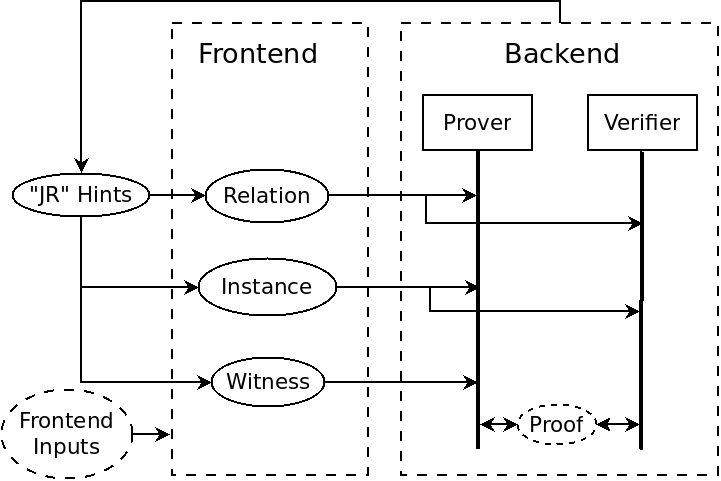
\includegraphics[width=0.75\textwidth,center]{ir-dataflow.png} \\

In its simplest form, the relation is a list of gate directives, each with an output wire and two input wires.
The gates and their connections through wires form a circuit.
This simple form is useful for streaming, where the proof system may consume a gate, process it, and immediately discard everything except the output wire.
These simple circuits can process wire values in two fields, either $GF(p)$ (``arithmetic'') or $GF(2)$ (``boolean'').
Beyond this simple form, the IR adds features for expressing uniformity in the circuit.
These features may be toggled on or off for a given relation, either enabling greater expressiveness, or guaranteeing the simple stream processing.
The first of these features is ``function-gates'' which encapsulate functionalities to be reused.
``For-loops'' repeat a sub-circuit for a fixed number of repetitions.
Lastly ``switch-case statements'' enable private conditions to be expressed directly in the IR.
These constructs both compact a relation and allow proof systems to quickly recognize structures and in some cases amortize computational effort.\\

\subsection{Concrete IR Formats}
This specification defines two forms, to resolve conflicting usage patterns between human and computer use cases.
To avoid ambiguity during translation from binary to text or vice-versa, special care must be taken to ensure that the text and binary formats remain isomorphic.
Specifically, every element defined by one format has an equivalent in the other format.\\

\begin{itemize}
  \item Text format - For human use during education, demonstration, and development.
  \item Binary format - For automated use in a performance critical environment.
\end{itemize}

\subsection{IR Validity and Semantics}\label{ir_validity}
In addition to isomorphic structure, both formats should have the same semantics.
This specification considers a few levels of validity, ranging from syntax and recognition through the acceptance of a proof given in the IR.
Each of the following validities is considered successive over the prior.

\begin{enumerate}
    \item \textbf{Syntactic Validity:} If a resource matches the syntactic constraints of either the Text (section \ref{text}) or Binary (section \ref{binary}) formats, then it is syntactically valid.\\
    \item \textbf{Resource Validity:} Each resource may be \textit{well-formed} if it, in isolation, satisfies constraints given in section \ref{text}.
    \begin{itemize}
        \item \textbf{Relation Well-formedness:} Satisfied mainly by its gates being topologically ordered, and in single static assignment (SSA) form.
        \item \textbf{Instance Well-formedness} and \textbf{Witness Well-formedness:} In isolation, the validity of these resources is indicated by each value being a member of the field.
    \end{itemize}
    \item \textbf{Evaluation Validity:} Considers all three resources together by evaluating each directive of the relation, consuming each value from the instance and witness streams, and checking that each \texttt{\$assert\_zero} directive carries the value $0$. If this is the case, then statement has a valid set of witness values that evaluate the circuit. In other words, when passed through a ZK backend system, the proof generated would be verified.
\end{enumerate}

Resource and Evaluation Validities may be collectively referred to as \textit{semantics}.

\subsection{IR Tooling (Informational only)}
We will briefly describe a few software suites for working with the SIEVE IR.
They are overviewed for informational purposes only, and their inclusion is not to be construed as an endorsement of either.

\textit{WizToolKit} is a toolkit and a library designed for working with the SIEVE IR in C++.
It includes parsing APIs for both the text and binary formats along with tools for checking \textit{resource validity} and \textit{evaluation validity} (\texttt{wtk-firealarm}), converting between the text and binary formats (\texttt{wtk-press}), and visualizing relations in graph form (\texttt{wtk-viz}).
\textit{WizToolKit} can be found in the \href{https://github.com/stealthsoftwareinc/wiztoolkit}{WizToolKit Repository}.\\

\textit{zkInterface-SIEVE} is an implementation of the FlatBuffers-based SIEVE IR and a set of tools used to enable interoperability between teams. The library extends the open-source \href{https://github.com/QED-it/zkinterface} library, which integrates several R1CS frontends and backends.
It includes API for producing and consuming relations in the IR binary format, and allows for parsing and printing JSON and YAML textual formats. The library includes a \texttt{validator} tool for checking \textit{resource validity}, an \texttt{evaluator} tool for checking \textit{evalutation validity}, a \texttt{metrics} tool for checking different stats about the circuit,  as well as converting to and from the existing \textit{zkInterface} R1CS relations.
\textit{zkInterface-SIEVE} can be found in the \href{https://github.com/QED-it/zkinterface-ir}{zkInterface-sieve repository}.\\

\newpage
\section{Example}\label{example}
A few samples of the SIEVE IR are given in this section.

\subsection{Point on Curve}\label{ex_ir0}
The following table shows an example arithmetic circuit.
The relation, instance, and witness are shown in their own columns.
The header resource is shown as an element of each of the other resources. \\

{
\lstset{language=ir}
\lstset{basicstyle=\scriptsize}
\noindent
\begin{tabularx}{\textwidth}{|X|X|X|}
\hline
\textbf{Relation} & \textbf{Instance} & \textbf{Witness} \\
\hline
This relation will check that a given point is a point on a Montgomery curve.\newline
$By^2 = x^3 + Ax^2 +x$
& A, and B, defining the curve are given as the instance -- available to both Prover and Verifier.
& x, and y, the point on the curve are the witness -- available only to the Prover. \\
\hline
%% Trail every newline in the listing with ^^j, otherwise the newline gets stripped by tabular.
\begin{lstlisting}^^J
// Header Start^^J
version 1.0.0;^^J
field^^J
  characteristic 97^^J
  degree 1;^^J
// Header End^^J
relation^^J
gate_set: arithmetic;^^J
features: simple;^^J
@begin^^J
$2 <- @short_witness; // x^^J
$3 <- @mul($2, $2); // x^2^^J
$4 <- @mul($2, $3); // x^3^^J
$0 <- @instance; // A^^J
$5 <- @mul($3, $0); // Ax^2^^J
$6 <- @add($4, $5);^^J
$7 <- @add($6, $2); // RHS^^J
@delete($0);^^J
@delete($2, $6);^^J
$8 <- @short_witness; // y^^J
$9 <- @mul($8, $8); // y^2^^J
$1 <- @instance; // B^^J
$10 <- @mul($9, $1); // LHS^^J
@delete($8, $9);^^J
$11 <- @mulc($7,<96>);^^J
$12 <- @add($11,$10);^^J
@assert_zero($12);^^J
@end^^J
\end{lstlisting} &
\begin{lstlisting}^^J
// Header Start^^J
version 1.0.0;^^J
field^^J
  characteristic 97^^J
  degree 1;^^J
// Header End
^^J
instance @begin^^J
  < 15 > ;^^J
  < 4 > ;^^J
@end^^J
\end{lstlisting} &
\begin{lstlisting}^^J
// Header Start^^J
version 1.0.0;^^J
field^^J
  characteristic 97^^J
  degree 1;^^J
// Header End
^^J
short_witness @begin^^J
  < 2 > ;^^J
  < 39 > ;^^J
@end^^J
\end{lstlisting} \\
\hline
\end{tabularx}
}

\subsection{Fibonacci}\label{ex_ir1}
These excerpts of IR code calculate the first ten (10) Fibonacci numbers.
Notably, the number of repetitions is \textit{not} private, it is a constant of the circuit.
Two versions are presented, one using an anonymous function as the body of the for-loop, another using a named function.\\

\subsubsection*{Anonymous For-Loop Body}
\lstset{language=ir}
\begin{lstlisting}
version 1.0.0;
field characteristic 97 degree 1;
relation
gate_set: arithmetic;
features: @for;
@begin
$0 <- <1>;
$1 <- <1>;
$2...$10 <- @for i @first 2 @last 10
  $i <- @anon_call($(i - 1), $(i - 2),
      @instance: 0, @short_witness: 0)
    $0 <- @add($1, $2);
  @end
@end
@end
\end{lstlisting}

\subsubsection*{Named For-Loop Body}
\lstset{language=ir}
\begin{lstlisting}
version 1.0.0;
field characteristic 97 degree 1;
relation
gate_set: arithmetic;
features: @function, @for;
@begin
@function(add_2, @out: 1, @in: 2,
    @instance: 0, @short_witness: 0)
  $0 <- @add($1, $2);
@end
$0 <- <1>;
$1 <- <1>;
$2...$10 <- @for i @first 2 @last 10
  $i <- @call(add_2, $(i - 1), $(i - 2));
@end
@end
\end{lstlisting}

\subsection{Matrix Multiplication}
This example demonstrates the multiplication of two matrices.
It reads matrix $M$ from the instance and matrix $N$ from the witness.
It also reads $C$ from the instance.
Then it computes $C'$ as $M*N$ and asserts that $C=C'$.\\

\begin{lstlisting}
version 1.0.0;
field characteristic 97 degree 1;
relation
gate_set:arithmetic;
features:@for,@function;
@begin
@function(sum, @out: 1, @in: 4, @instance: 0, @short_witness: 0)
  // out: $0
  // in: $1 ... $4
  $5 <- @add($1, $2);
  $6 ... $6 <- @for i @first 2 @last 2
    $(i + 4) <- @anon_call($(1 + i), $(3 + i),
        @instance: 0, @short_witness: 0)
      $0 <- @add($1, $2);
    @end
  @end
  $0 <- @add($4, $6);
@end

// M (3x4): $0...$11 (instance)
// N (4x5): $27...$46 (witness)
// C (3x5): $12...$26 (instance)
// C' (3x5): $47...$61

// Computes the product C':=M*N, and checks that C'==C

$0 ... $11 <- @for i @first 0 @last 11
  $i <- @anon_call(@instance: 1, @short_witness: 0)
    $0 <- @instance;
  @end
@end
$12 ... $26 <- @for i @first 12 @last 26
  $i <- @anon_call(@instance: 1, @short_witness: 0)
    $0 <- @instance;
  @end
@end
$27 ... $46 <- @for i @first 27 @last 46
  $i <- @anon_call(@instance: 0, @short_witness: 1)
    $0 <- @short_witness;
  @end
@end

$47 ... $61 <- @for i @first  0 @last 2
  $(47 + (i * 5)) ... $(51 + (i * 5)) <- @anon_call(
      $0 ... $11, $27 ... $46,
      @instance: 0, @short_witness: 0)
    // C'[i][...]: $0 ... $4
    // M: $5 ... $16
    // N: $17 ... $36
    $0 ... $4 <- @for j @first 0 @last 4
      $j <- @anon_call($5 ... $16, $17... $36,
          @instance: 0, @short_witness: 0)
        // C'[i][j]: $0
        // M: $1 ... $12
        // N: $13 ... $32
        $33 ... $36 <- @for k @first 0 @last 3
          $(k + 33) <- @anon_call(
              $(1 + ((i * 4) + k)), $(13 + ((k * 5) + j)),
              @instance: 0,@short_witness: 0)
            $0 <- @mul($1, $2);
          @end
        @end
        $0 <- @call(sum, $33 ... $36);
      @end
    @end
  @end
@end

// Check that C' == C
@for i @first 0 @last 2
  @anon_call(
      $((i * 5) + 12) ...$((i * 5) + 16),
      $((i * 5) + 47) ... $((i * 5) + 51),
      @instance: 0, @short_witness: 0)
    // C[i][...]: $0 ... $4
    // C'[i][...]: $5 ... $9
    @for j @first 0 @last 4
      @anon_call($j, $(j + 5), @instance: 0, @short_witness: 0)
        $2 <- @mulc($0, < 96 >);
        $3 <- @add($1, $2);
        @assert_zero($3);
      @end
    @end
  @end
@end
@end

\end{lstlisting}

%%%%
\newpage
\section{IR Overview and Abstract Syntax}\label{overview}
This section will describe the SIEVE IR at an overview level and should be sufficient to grant a workable understanding of the IR.
Section \ref{text} will provide authoritative textual syntax and IR semantics; Section \ref{binary} will provide binary syntax.
Mentioned previously, the IR has three (3) ``resources'' which may be thought of as files but could also be provided via other methods -- e.g. streams, shared memory, and so on.
These resources take the R(x; w) form: R is the relation, x is the instance, and w is the witness. \\

The IR's relation represents a circuit using sequence of directives to manage a sparsely populated lists of wire values.
A value is described by its index in the list, and most directives will insert a new value at an output index.
A wire's index is represented as an integer in the range of $0$ and $2^{64}-1$.
Although a directive may reference or insert a value at any index, using sequential indexes can improve performance.
The lists are considered sparse for two reasons. 
First, wires may be removed from the list to conserve memory.
Second, the minimal constraints on output index usage means that gaps may form in the wires list, although this is discouraged.\\

The instance and witness resources are streams of values.
Certain directives in the relation will consume a value from either stream.\\

\lstset{language=ir}
\lstset{frame=single}
\lstset{escapechar=\#}

\newcommand{\asTemplate}[1]{{\color{SyntaxGreen}{\textit{\{\texttt{#1}\}}}}}
\newcommand{\asRepeat}[0]{{\color{SyntaxGreen}{...}}}

This overview uses ``template'' texts, surrounded with boxes, and where ``template expressions'' may be repeated and replaced by concrete expressions described elsewhere.
In general, whitespace is optional and ignored, except for a single whitespace element delimiting non-obvious token sequences.
Template expressions are italicized with surrounding delimiters with dark green text, for example \asTemplate{expression}.
All template expressions will be described as appropriate literal values, or sub expressions.
Repetition of a template expression is indicated with an ellipsis (\asRepeat), also in green.
Tables following each template will describe the semantics of each template.\\

\subsection{Resource Header Overview}\label{header_overview}
The first component of the IR is a header block with evaluation parameters for the circuit.
The header is shared by all resources.
There are two parameters defined by the header: a version number for quick recognition of the IR, and the computation field.\\

\begin{lstlisting}
version #\asTemplate{major}#.#\asTemplate{minor}#.#\asTemplate{patch}#;

field
  characteristic #\asTemplate{p}#
  degree 1;
\end{lstlisting}

\subsubsection*{Header Semantics}

\noindent
\begin{tabularx}{\textwidth}{|p{1in}|p{1in}|X|}
  \hline
  \textbf{Template Expression} & \textbf{Name} & \textbf{Description} \\
  \hline
  \asTemplate{major}\newline
  \asTemplate{minor}\newline
  \asTemplate{patch}\newline & Version & The version of the IR is given in \href{https://semver.org/}{semantic version form}.
  This must match one of the versions given in the \nameref{history} section of this document. \newline
  \newline
  Syntactically, these parameters must be positive unbounded integers, in decimal form, with no leading zeros.\\
  \hline
  \asTemplate{p} & Field & The field governs the domain in which proofs may be expressed.
  It may be either $GF(p)$ or $GF(2)$ (a special case of the former).
  The syntax gives a characteristic ($p$), and a degree ($n$) which would describe a field $GF(p^n)$.
  However the degree is fixed to one (1).\newline
  \newline
  The $p$ variable may be an unbounded integer, and must be prime. \\
  \hline
\end{tabularx}

\subsection{Instance and Short Witness Overview}\label{ins_wit_overview}
Syntactically each of the instance and short witness is a sequence of field elements, acting as a stream.
Certain directives in the relation will consume a value from one of these streams.
If values in either stream are exhausted this is a failure of \textit{evaluation validity}.
If values remain in a stream after processing then this is also an \textit{evaluation invalidity}.\\

\begin{lstlisting}
#\asTemplate{header}#

#\asTemplate{type}# @begin
  < #\asTemplate{c}# > ; #\asRepeat#
@end
\end{lstlisting}

\subsubsection*{Instance and Witness Semantics}

\noindent
\begin{tabularx}{\textwidth}{|p{1in}|X|p{1.5in}|p{1.75in}|}
  \hline
  \textbf{Template Expression}
  & \textbf{Description}
  & \textbf{Syntactic\newline Constraints}
  & \textbf{Semantic\newline Constraints} \\
  \hline
  \asTemplate{header}
  & A header, as described in section \ref{header_overview}, is required here.
  & See section \ref{header_overview}.
  & The $\{p\}$ variable is captured in this section. \\
  \hline
  \asTemplate{type}
  & Indicates whether this resource is the instance or witness.
  & Must be the exact text \texttt{instance} or \texttt{short\_witness}. & \\
  \hline
  \asTemplate{c}\asRepeat
  & Each \asTemplate{c} is a literal constant specified as a gate input.
  & A numeric literal, which is syntactically positive and unbounded.
  & Must be in the range of $0$ up to $\{p\}$. \\
  \hline
\end{tabularx}

\subsection{Relation Overview: Structure, Gate Set, and Feature Toggles}\label{rel_structure_overview}
The relation starts by describing its own contents, first by which gates it may use (the \textit{gate set}) then by which uniformity features it may use (\textit{feature toggles}).
Following these is a list of function gate declarations, a list of the named function gates allowed in the relation, along with function gate definitions.
Lastly is the body of  the relation, the list of directives making up the circuit.\\

\begin{lstlisting}
#\asTemplate{header}#
relation 
gate_set: #\asTemplate{gateset}#;
features: #\asTemplate{features}#;
@begin
  #\asTemplate{functions}\asRepeat#
  #\asTemplate{directive}\asRepeat#
@end
\end{lstlisting}

Each template expression is described in this table.\\

\noindent
\begin{tabularx}{\textwidth}{|p{1.25in}|p{1in}|X|}
  \hline
  \textbf{Template \newline Expression} & \textbf{Name} & \textbf{Description} \\
  \hline
  \asTemplate{header}
  & Header
  & A header, as described in section \ref{header_overview}, is required here. \\
  \hline
  \asTemplate{gateset}
  & \textit{Gate set}
  & The \textit{gate set} describes the allowable gate directives of the circuit.
  The actual gate directives will be described in section \ref{function_gate_overview}.
  There are two \textit{canonical gate sets}, either \texttt{arithmetic} or \texttt{boolean}.
  If a \texttt{canonical gate set} is not desired, then a \textit{partial gate set} may described as the enumeration of gate names.\newline
  \newline
  A \textit{partial gate set} is defined by a comma separated subset of the gates from a \textit{canonical gate set}.
  For \texttt{arithmetic}, these would be \texttt{@add}, \texttt{@addc}, \texttt{@mul}, and \texttt{@mulc}; and for \texttt{boolean} gates these would be \texttt{@and}, \texttt{@not}, and \texttt{@xor}.
  If an \textit{partial gate set} enumeration were empty, it would be considered a semantic error.
  \\
  \hline
  \asTemplate{features}
  & \textit{Feature Toggles}
  & The feature toggles are a list of optional features which may be enabled or disabled by their presence.
  If a feature is present, it must appear in a comma separated set. The allowed features are \texttt{@function}, \texttt{@for}, and \texttt{@switch}\newline
  \newline The toggles for \texttt{@for} and \texttt{@switch} each describes whether for loops (subsection \ref{loop_overview}) or switch-case statements (subsection \ref{switch_overview}) are enabled.
  The toggle for \texttt{@function} indicates whether function gates (subsection \ref{function_gate_overview}) are allowed, except for anonymous functions within the body of a for loop or switch-case statement.
  If no features are enabled, then the keyword \texttt{simple} should take the feature list's place.\newline
  \newline
  Unless the \textit{feature toggle} is \texttt{simple}, wires between $2^{63}$ and $2^{64} - 1$ are reserved as ``ephemeral wires'', meaning that the frontend may not emit them.
  Instead, the backend may insert them as needed.\\
  \hline
  \asTemplate{functions}\asRepeat
  & Function Gate Declarations
  & This is a list of function gate declarations.
  Each declares a named function gate which may be used as a \asTemplate{directive}.
  Further description will be given in subsection \ref{function_invoke_overview}\\
  \hline
  \asTemplate{directive}\asRepeat & Directives & This is a list of directives, each directive will be described in further subsections \ref{rel_gates_overview}, \ref{function_gate_overview}, \ref{loop_overview}, and \ref{switch_overview}. \\
  \hline
\end{tabularx}

\subsection{Relation Overview: Simple Gate Directives}\label{rel_gates_overview}
Most of the relation is described through lists of directives.
``Gate directives'' perform calculations on their inputs and produce an output.
In general, gate directives will look like the assignment of the calculation's result to a wire.
There are three allowed forms for a gate directive.\\

\begin{itemize}
  \item \textbf{Binary} directives have two wire inputs, and one output. They are written as
  \begin{lstlisting}
  $#\asTemplate{x}# <- #\asTemplate{calculation}# ( $#\asTemplate{y}# , $#\asTemplate{z}# );
  \end{lstlisting}
  \item \textbf{Binary constant} directives have one wire input, one constant input, and one output. They are written as
  \begin{lstlisting}
  $#\asTemplate{x}# <- #\asTemplate{calculation}# ( $#\asTemplate{y}# , < #\asTemplate{c}# > );
  \end{lstlisting}
  \item \textbf{Unary} directives have one wire input, and one output. They are written as
  \begin{lstlisting}
  $#\asTemplate{x}# <- #\asTemplate{calculation}# ( $#\asTemplate{y}# );
  \end{lstlisting}
\end{itemize}

The allowed \asTemplate{calculation}s for each directive vary by the profile given in the header.
Each of the given function names can be considered a keyword in the IR language. \\

\begin{itemize}
  \item Under the \texttt{boolean} \textit{canonical gate set}, the following calculations are defined.
  \begin{itemize}
    \item \texttt{@and} is a binary directive which computes logical and.
    \item \texttt{@xor} is a binary directive which computes logical exclusive or.
    \item \texttt{@not} is a unary directive which computes logical negation.
  \end{itemize}
  \item Under the \texttt{arithmetic} \textit{canonical gate set}, the following calculations are defined.
  \begin{itemize}
    \item \texttt{@mul} is a binary directive which computes field multiplication.
    \item \texttt{@add} is a binary directive which computes field addition.
    \item \texttt{@mulc} is a binary constant directive which computes field multiplication.
    \item \texttt{@addc} is a binary constant directive which computes field addition.
  \end{itemize}
\end{itemize}

In both profiles, five special directives, called the \emph{common directives}, are allowed: Copy, Assignment, Assert Zero, Input (instance and short\_witness), and Deletion, as indicated below.
Regardless of \textit{gate set}, these directives are always allowed.
\begin{itemize}
  \item \textbf{Copy} will duplicate the value of one variable into another variable.
  \begin{lstlisting}
  $#\asTemplate{x}# <- $#\asTemplate{y}#;
  \end{lstlisting}
  \item \textbf{Assignment} will give one variable a constant value.
  \begin{lstlisting}
  $#\asTemplate{x}# <- < #\asTemplate{c}# >;
  \end{lstlisting}
  \item \textbf{Assert Zero} will check that a variable is equivalent to zero (0), otherwise it constitutes an \textit{evaluation invalidity}.
  \begin{lstlisting}
  @assert_zero( $#\asTemplate{y}# );
  \end{lstlisting}
  \item \textbf{Input} directives have a single output wire, and read the next value of the named stream.
    The \asTemplate{input-stream} may be either of \verb|@short_witness| or \verb|@instance|, indicating which of the input streams to read from.
    These may be considered keywords of the IR language.
  \begin{lstlisting}
  $#\asTemplate{x}# <- #\asTemplate{input-stream}#;
  \end{lstlisting}
  \item \textbf{Deletion} will remove a wire or a range of wires from the wires list.
  \begin{lstlisting}
  @delete( $#\asTemplate{y}# );
  @delete( $#\asTemplate{a}#, $#\asTemplate{b}# );
  \end{lstlisting}
\end{itemize}

The following table describes each of the template expressions used in this subsection.\\

\noindent
\begin{tabularx}{\textwidth}{|p{1in}|X|p{1.5in}|p{1.75in}|}
  \hline
  \textbf{Template Expression}
  & \textbf{Description}
  & \textbf{Syntactic\newline Constraints}
  & \textbf{Semantic\newline Constraints} \\
  \hline
  \asTemplate{x}
  & A single directive output wire specified as a 0-based index.
  & A numeric literal in the range of $[0; 2^{64})$.
  & No \asTemplate{x} wire may appear more than once, even if the \asTemplate{x} has been deleted previously.\newline
  \newline
  Unless the \textit{feature toggle} is \texttt{simple}, \asTemplate{x} must not exceed $2^{63}$\\
  \hline
  \asTemplate{y} \newline
  \asTemplate{z}
  & A single directive input wire specified as a 0-based index.
  & A numeric literal in the range of $[0; 2^{64})$.
  & A wire \asTemplate{y} or \asTemplate{z} must have been assigned a value before appearing as a \asTemplate{y} or a \asTemplate{z} and must not have been previously deleted.\newline
  \newline
  Unless the \textit{feature toggle} is \texttt{simple}, \asTemplate{y} or \asTemplate{z} must not exceed $2^{63}$\\
  \hline
  \asTemplate{c}
  & A literal constant specified as a gate input.
  & A numeric literal which is syntactically an unbounded positive integer.
  & \asTemplate{c} must be in the range of $0$ up to but not including \asTemplate{p}. \\
  \hline
  \asTemplate{a}, \newline
  \asTemplate{b}
  & A range of wires starting at \asTemplate{a} and concluding at \asTemplate{b}, both inclusive.
  & A numeric literal in the range of $[0; 2^{64})$.
  & Each wire between \asTemplate{a} and \asTemplate{b} must have previously been assigned a value and must not have been previously deleted.\newline
  \newline
  Unless the \textit{feature toggle} is \texttt{simple}, no wire in this range must exceed $2^{63}$.\\
  \hline
\end{tabularx}

\subsection{Relation Overview: Function Gates}\label{function_gate_overview}
The function gate feature adds a function declaration and two directives to the IR.

\begin{description}[labelindent=0.375in]
    \item[Declaration] Declares a named function gate for later use.
      These must be listed together at the beginning of the relation.
    \item[Invocation] Invokes a previously declared function gate.
    \item[Anonymous Invocation] Define a function gate at the point of its invocation.
\end{description}

Should a backend wish not to support function gates directly, they may be ``inlined'', replacing their invocations with a copy of their body.
A procedure for this is outlined in section \ref{inlining}.\\

\subsubsection*{Function Gate Declaration}\label{function_declare_overview}
Function gates are declared ahead of time and invoked later.
Their declarations indicate the number of wires entering and exiting the function-gate, as well as the number of instance and short witness values it will consume.\\

\begin{lstlisting}
@function(#\asTemplate{name}#, @out: #\asTemplate{out}#, @in: #\asTemplate{in}#,
    @instance: #\asTemplate{n\_instance}#, @short_witness: #\asTemplate{n\_s\_witness}#)
  #\asTemplate{directives}\asRepeat#
@end
\end{lstlisting}

\subsubsection*{Function Gate Declaration Semantics}

\noindent
\begin{tabularx}{\textwidth}{|p{1.25in}|X|p{1.5in}|p{1.375in}|}
  \hline
  \textbf{Template\newline Expression}
  & \textbf{Description}
  & \textbf{Syntactic\newline Constraints}
  & \textbf{Semantic\newline Constraints} \\
  \hline
  \asTemplate{name}
  & The name by which this function gate will be referenced.
  & This is a C-like identifier, but may also use \texttt{.} or \texttt{::} for grouping similar functions.
  & The name must not have previously been used in another function gate declaration. \\
  \hline
  \asTemplate{out}
  & The number of outputs wires from the subcircuit.
  & Integer literal between $0$ and $2^{64}-1$.
  & Gate directives may output on wires $0$ through $\asTemplate{out} - 1$ to assign the subcircuit's output wires.\\
  \hline
  \asTemplate{in}
  & The number of input wires from the subcircuit.
  & Integer literal between $0$ and $2^{64}-1$.
  & Gate directives may input from wires $\asTemplate{out}$ through $\asTemplate{in} + \asTemplate{out} -1$ to consume the subcircuit's input wires.\\
  \hline
  \asTemplate{n\_instance}
  & The number of instance values consumed the subcircuit.
  & Integer literal between $0$ and $2^{64}-1$.
  & \asTemplate{directives}\asRepeat\  must have enough \texttt{@instance} directives or function gate invocations so that the \texttt{@instance} directive count plus all the invocations' \asTemplate{n\_instance}s is \asTemplate{n\_instance}, exactly.\\
  \hline
  \asTemplate{n\_s\_witness}
  & The number of short witness values consumed by the subcircuit.
  & Integer literal between $0$ and $2^{64}-1$.
  & \asTemplate{directives}\asRepeat\ must have enough \texttt{@short\_witness} directives or function gate invocations so that the \texttt{@short\_witness} directive count plus all the invocations' \asTemplate{n\_s\_witness}s is \asTemplate{n\_s\_witness}, exactly.\\
  \hline
  \asTemplate{directives}\asRepeat
  & A list of directives (other than more function gate definitions) forming the body of the function gate.
  & These are the same directives from IR0 as allowed by the \textit{gate set}. Additionally, IR1 directives may be used, except for more function gate declarations.
  & Gate directives may assign to wires $\asTemplate{in} + \asTemplate{out}$ or higher to create wires local to the subcircuit.\\
  \hline
\end{tabularx}

\subsubsection*{Function Gate Invocation}\label{function_invoke_overview}
A function gate may be invoked as follows.
An invocation may occur within the top-level circuit, or within a subcircuit.
Note however, if a function-gate is invoked from within a function-gate, it must have been declared lexically ahead of the current one, specifically preventing direct or indirect recursion.\\

\begin{lstlisting}
#\asTemplate{out-list}# <- @call(#\asTemplate{name}#, #\asTemplate{in-list}#);
\end{lstlisting}

If a function gate has no inputs or no outputs, then the invocation may take one of the following forms.
An invocation could also have no inputs and no output wires, presumably if it consumed from \texttt{@short\_witness} or \texttt{@instance} for input, and used \texttt{@assert\_zero} in lieu of output wires.\\

\begin{lstlisting}
@call(#\asTemplate{name}#, #\asTemplate{in-list}#);

#\asTemplate{out-list}# <- @call(#\asTemplate{name}#);

@call(#\asTemplate{name}#);
\end{lstlisting}

\subsubsection*{Function Gate Invocation Semantics}
\noindent
\begin{tabularx}{\textwidth}{|p{1.25in}|X|p{1.5in}|p{1.375in}|}
  \hline
  \textbf{Template\newline Expression}
  & \textbf{Description}
  & \textbf{Syntactic\newline Constraints}
  & \textbf{Semantic\newline Constraints} \\
  \hline
  \asTemplate{name}
  & The name of the function to be invoked.
  & This is a C-like identifier, but may also use \texttt{.} or \texttt{::} for grouping similar functions.
  & The name must have previously been used as a function gate declaration.\\
  \hline
  \asTemplate{out-list}
  & A list of wires which will connect the output wires of the subcircuit.
  & Must be a wire list, as described below.
  & The number of wires in the list must be equal to the \asTemplate{out} parameter of the function gate declaration.
  Each wire in the list must be distinct.
  \newline\newline
  The wires in this list must not have previously been assigned.
  These wires will be assigned after the invocation.\\
  \hline
  \asTemplate{in-list}
  & A list of wires which will connect the output wires of the subcircuit.
  & Must be a wire list, as described below.
  & The number of wires in the list must be equal to the \asTemplate{in} parameter of the function gate declaration.
  Wires in this list may be duplicates, although this is not recommended.
  \newline\newline
  The wires in this list must have previously been assigned.\\
  \hline
\end{tabularx}

The wire list syntax used for \asTemplate{out-list} and \asTemplate{in-list} are lists of either single indexes or index ranges.
Multiple indexes and index ranges may be separated by commas.

\begin{description}[labelindent=0.375in]
    \item[Single] \texttt{\$\asTemplate{x}}, where \asTemplate{x} is an integer literal.
    The wire list will contain the wire \asTemplate{x}.
    \item[Range] \texttt{\$\asTemplate{x}...\$\asTemplate{y}}, where \asTemplate{x} and \asTemplate{y} are integer literals.
    The wire list will contain every wire between \asTemplate{x} and \asTemplate{y} (inclusive).
\end{description}

\subsubsection*{Function Gate Invocation Example}
This example demonstrates a simple function gate computing the sum of four inputs.

\begin{lstlisting}
version 1.0.0;
field characteristic 97 degree 1;
relation
gate_set: arithmetic;
features: @function;
@begin
  @function(add_4, @out: 1, @in: 4,
      @instance: 0, @short_witness: 0)
    $5 <- @add($1, $2);
    $6 <- @add($3, $4);
    $0 <- @add($5, $6);
  @end

  $0 <- @short_witness;
  $1 <- @instance;
  $2 <- @short_witness;
  $3 <- @instance;
  $4 <- @call(add_4, $0...$3);
  @assert_zero($4);
@end
\end{lstlisting}

\subsubsection*{Anonymous Invocations}
An anonymous invocation declares an unnamed function gate, and invokes it in the same directive.
It has the following form.\\

\begin{lstlisting}
#\asTemplate{out-list}# <- @anon_call(#\asTemplate{in-list}#,
    @instance: #\asTemplate{n\_instance}#, @short_witness: #\asTemplate{n\_s\_witness}#)
  #\asTemplate{directives}\asRepeat#
@end
\end{lstlisting}

Just like a named function invocation, an anonymous function may have no inputs or no outputs.

\begin{lstlisting}
@anon_call(#\asTemplate{in-list}#, @instance: #\asTemplate{n\_instance}#,
    @short_witness: #\asTemplate{n\_s\_witness}#)
  #\asTemplate{directives}\asRepeat#
@end

#\asTemplate{out-list}# <- @anon_call(@instance: #\asTemplate{n\_instance}#,
    @short_witness: #\asTemplate{n\_s\_witness}#)
  #\asTemplate{directives}\asRepeat#
@end

@anon_call(@instance: #\asTemplate{n\_instance}#, @short_witness: #\asTemplate{n\_s\_witness}#)
  #\asTemplate{directives}\asRepeat#
@end
\end{lstlisting}

The following template expressions are related to those of the Function Gate Declaration (\ref{function_declare_overview}) or Function Gate Invocation (\ref{function_invoke_overview}).

\noindent
\begin{tabularx}{\textwidth}{|p{1.5in}|X|}
  \hline
  \textbf{Template\newline Expression} & \textbf{Explanation} \\
  \hline
  \asTemplate{name} & The \asTemplate{name} is not used by an anonymous invocation. \\
  \hline
  \asTemplate{out}, \asTemplate{in} & These template expressions of a Declaration are replaced with the length of the \asTemplate{out-list} and \asTemplate{in-list} wire lists. \\
  \hline
  \asTemplate{n\_instance}, \asTemplate{n\_s\_witness} & These have the same usage in a Declaration and an Anonymous Invocation. \\
  \hline
  \asTemplate{directives}\asRepeat & This has the same usage in  a Declaration and an Anonymous Invocation. \\
  \hline
  \asTemplate{out-list} \asTemplate{in-list} & These have the same usage in an Invocation and an Anonymous Invocation. \\
  \hline
\end{tabularx}

\subsubsection*{Anonymous Invocation Example}
This example demonstrates an anonymous function computing the sum of four inputs.

\begin{lstlisting}
version 1.0.0;
field characteristic 97 degree 1;
relation
gate_set: arithmetic;
features: @function;
@begin
  $0 <- @short_witness;
  $1 <- @instance;
  $2 <- @short_witness;
  $3 <- @instance;
  $4 <- @anon_call($0...$3, @instance: 0, @short_witness: 0)
    $5 <- @add($1, $2);
    $6 <- @add($3, $4);
    $0 <- @add($5, $6);
  @end
  @assert_zero($4);
@end
\end{lstlisting}

\subsection{Relation Overview: For Loops}\label{loop_overview}
A for loop repeats the invocation of a function gate.
The invocation may be anonymous, but this is not required.
It has the following form.\\

Should a backend wish not to support for loops directly a procedure for ``unrolling'' a loop is described in section \ref{unrolling}.\\

\begin{lstlisting}
#\asTemplate{assign-list}# <- @for #\asTemplate{iterator}# @first #\asTemplate{first}# @last #\asTemplate{last}#
  #\asTemplate{invocation}#
@end
\end{lstlisting}

A for loop may omit the \asTemplate{assign-list} so long as its \asTemplate{invocation} has no output wires. In this case the \asTemplate{invocation} must also not have an \asTemplate{out-list}.\\

\begin{lstlisting}
@for #\asTemplate{iterator}# @first #\asTemplate{first}# @last #\asTemplate{last}#
  #\asTemplate{invocation}#
@end
\end{lstlisting}

\subsubsection*{For Loop Semantics}

\begin{tabularx}{\textwidth}{|p{1.125in}|X|p{1.375in}|p{1.75in}|}
  \hline
  \textbf{Template\newline Expression}
  & \textbf{Description}
  & \textbf{Syntactic\newline Constraints} & \textbf{Semantic\newline Constraints} \\
  \hline
  \asTemplate{assign-list}
  & A list of wires, in the scope containing the for loop, which are assigned by the for loop.
  & The same wire list form as used by Function Gate Invocation (\ref{function_invoke_overview}).
  & Before the loop, all wires in the list must be unassigned. After the loop all of them will have been assigned. \\
  \hline
  \asTemplate{iterator}, \asTemplate{first}, \asTemplate{last}
  & These control the number of iterations of the loop.\newline\newline
  \asTemplate{iterator} is a loop iterator (see below), while \asTemplate{first} and \asTemplate{last} are start and stop conditions.
  & \asTemplate{iterator} is an identifier (see below).
  \newline\newline
  \asTemplate{first} and \asTemplate{last} may be iterator expressions (see below).
  & \asTemplate{iterator} increments by one (1) on each iteration of the loop.\newline\newline
  On the first iteration, \asTemplate{iterator} carries the value \asTemplate{first}, and on the last it carries the value \asTemplate{last}. \\
   \hline
  \asTemplate{invocation} (and transitively \asTemplate{out-list} and \asTemplate{in-list})
  & This is a function gate invocation, anonymous or not.
  & The wire indexes in the invocation's \asTemplate{out-list} and \asTemplate{in-list} may be replaced with iterator expressions (see below).
  & The union of each iteration's \asTemplate{out-list} must form an equivalent set to the \asTemplate{assign-list}.
  Each iteration's \asTemplate{out-list} must be distinct from that of each other iteration. \\
  \hline
\end{tabularx}

\subsubsection*{Iterator Expressions}\label{overview-iterators}
Iterator expressions enable the input and output wires of a function gate invocation to differ on each iteration of the loop.
Each iterator expression is a simple arithmetic expressions using the loop \asTemplate{iterator}s of any lexically containing loop.
The expressions replace wire indexes for the \asTemplate{invocation}'s inputs and outputs.
An iterator expression can take one of the following forms, and represents the index of a wire, using integers between $0$ and $2^{64}-1$.
Loop \asTemplate{iterator}s have lexical scope.
Functionally, this means that on scope boundaries entering an anonymous function they are preserved, but entering a named function they are not.
For further clarity refer to section \ref{for_loops_text}. \\

\begin{itemize}
    \item A numeric constant.
    \item A ``loop iterator'', which refers to the value of a loops iteration counter.
    Syntactically this is a C-style identifier, but may also use \texttt{.} or \texttt{::} for grouping similar functions. See Appendix \ref{textblocks} for details.
    \item An expression of ``sub-expressions''. This takes the form \texttt{(\asTemplate{a} \asTemplate{op} \asTemplate{b})}. Where \asTemplate{a} and \asTemplate{b} are ``sub- expressions'', and \asTemplate{op} is one of the following operations.
    The operations have wraparound behavior from $2^{64}-1$ to $0$.
    \begin{itemize}
        \item \texttt{+}: integer addition.
        \item \texttt{-}: integer subtraction.
        \item \texttt{*}: integer multiplication.
    \end{itemize}
    \item A division constant expression. This takes the form \texttt{\asTemplate{a} / \asTemplate{b}} where \asTemplate{a} is a ``sub-expression'' and \asTemplate{b} is a numeric constant. The result is the 64-bit unsigned integer quotient.
\end{itemize}

\subsubsection*{Examples}
Here are a few example ``iterator-expressions'', as well an example of Fibonacci.
Note that for Fibonacci, the ``$n$'' is a public constant (the bounds of the loop).

\begin{itemize}
    \item \texttt{\$123} is the exact wire.
    \item \texttt{\$i} or \texttt{\$(i + 123)} indexes an ``array'' within a for-loop.
    \item \texttt{\$((i * 10) + j)}  indexes a ``square array'' within a pair of for-loops.
\end{itemize}

\begin{lstlisting}
$2...$10 <- @for i @first 2 @last 10
  $i <- @anon_call($(i - 1), $(i - 2),
      @instance: 0, @short_witness: 0)
    $0 <- @add($1, $2);
  @end
@end
\end{lstlisting}

To clarify lexical \asTemplate{iterator} scoping consider the following two example nested loop excerpts.
The first nests using anonymous functions for the outer loop body.
The second uses a named function, and because some of the inner loop's iterator expressions use the outer loop's iterator, an error is caused.\\

\begin{lstlisting}
 /* ... */ <- @for i @first 0 @last 10
   /* ... */ <- @anon_call(/* ... */)
     @for j @first 0 @last 10
       $((i * 10) + j) <- @anon_call(/* ... */)
         /* ... */
       @end
   @end
 @end
\end{lstlisting}

The equivalent using named functions is however erroneous.\\

\begin{lstlisting}
@function(foo, /* ... */)
  /* ... */ <- @for j @first 0 @last 10
    $((i * 10) + j) <- @anon_call(/* ... */) // #{\color{red} Error}#
      /* ... */
    @end
  @end
@end

/* ... */ <- @for i @first 0 @last 10
  /* ... */ <- @call(foo, /* ... */)
@end
\end{lstlisting}

\subsection{Relation Overview: Switch-Case Statements}\label{switch_overview}
The switch-case directive grants the IR the capability to evaluate branches, as is ubiquitous in conventional computing.
However, in order to protect the the short witness, performance characteristics cannot always be mirrored.
If the length or structure of one branch differs from other branches, then the verifier could use such information to learn about the witness.
Thus, every branch is processed, and only the result of the matching branch is chosen as the ``selected'' result. \\

Should a backend wish not to support a switch-case directly, a procedure for conversion to a selection circuit, or ``multiplexing'', is described in section \ref{multiplexing}.\\

\begin{lstlisting}
#\asTemplate{assign-list}# <- @switch ( $#\asTemplate{condition}# )
  @case < #\asTemplate{case}# > : #\asTemplate{invocation}# 
  @case < #\asTemplate{case}# > : #\asTemplate{invocation}# 
  @case < #\asTemplate{case}# > : #\asTemplate{invocation}# 
  #\asRepeat#
@end
\end{lstlisting}



\subsubsection*{Switch-Case Semantics}
The \asTemplate{condition} is the wire index of an assigned wire, whose value is matched against each \asTemplate{case}.
Where the \asTemplate{condition}'s value matches a \asTemplate{case}, the corresponding \asTemplate{invocation}'s assignments are kept as the \asTemplate{assign-list}'s assignments.\\

If any two \asTemplate{case}s have the same value, then the relation is semantically invalid.
If the \asTemplate{condition} does not match any \asTemplate{case}, the witnessed statement is invalid.\\

\begin{tabularx}{\textwidth}{|p{1.125in}|X|p{1.375in}|p{1.75in}|}
  \hline
  \textbf{Template\newline Expression}
  & \textbf{Description}
  & \textbf{Syntactic\newline Constraints} & \textbf{Semantic\newline Constraints} \\
  \hline
  \asTemplate{assign-list}
  & A list of wires, in the scope containing the switch-case, which are assigned by the switch-case.
  & The same wire list form as used by Function Gate Invocation (\ref{function_invoke_overview}).
  & Before the switch-case, all wires in the list must be unassigned. Afterwards all of them will have been assigned. \\
  \hline
  \asTemplate{condition}, \asTemplate{case}
  & These select the ``selected'' case of the switch-case statement.
  & The \asTemplate{condition} is a wire-number, prefixed by \texttt{\$}, and in the range of $0$ through $2^{63}-1$.\newline
  \newline
  Each \asTemplate{case} is a field element, delimited with \texttt{<} and \texttt{>}.
  & The \asTemplate{condition} must have been previously assigned, and each \asTemplate{case} must be in the range of $0$ through $p-1$.
  No \asTemplate{case} may be duplicated within a same switch-case.\newline
  \newline
  If the \asTemplate{condition}'s value is not matched by a case, this is an \textit{evaluation invalidity}.
  \\
   \hline
  \asTemplate{invocation} (and transitively \asTemplate{out-list}, \asTemplate{in-list}, and \asTemplate{directives})
  & Each case is backed by a function gate invocation, either named or anonymous.
  & The \asTemplate{out-list} and \texttt{<-} are omitted from each invocation, otherwise, these are syntactically identical to a named or anonymous function-gate invocation.
  & The \asTemplate{assign-list} must have the same length as the \asTemplate{out-list} would have.
  The ``selected'' case's \asTemplate{out-list} is replaced with the \asTemplate{assign-list}, while each other case's \asTemplate{out-list} is replaced with wires which can be considered discarded.\newline
  \newline
  A \asTemplate{directive} which has side-effects must have special meaning described in subsection \ref{switch_side_effects_overview}.
  \\
  \hline
\end{tabularx}

\subsubsection*{Side-Effect Directives in a Switch-Case Statement}\label{switch_side_effects_overview}
As certain directives have effects other than assignment of wires, their semantics within a switch-case must be modified.
Specifically \texttt{@assert\_zero} and the input directives, \texttt{@instance} and \texttt{@short\_witness}, have altered semantics.\\

The \texttt{@assert\_zero} directive causes an \textit{evaluation invalidity} if its given wire does not carry the value zero (0).
This effect is undesirable in non-selected cases, thus the effect is disabled in the body of each case, except the selected case. \\

The input directives (\texttt{@instance} and \texttt{@short\_witness}) cause streams to be advanced on each occurrence, and each branch might use a different number of inputs.
If the IR were to match exactly the expectation of conventional branching, then differing stream consumption counts could reveal the switch condition, breaking zero-knowledge.
However, if the IR were to trace each branch and consume every input on each branch, this could be wasteful and preclude certain interesting optimizations.
Instead, the totality of the switch-case must consume the maximum number of inputs regardless of which case.
This could be implemented by duplicating the stream before each case (demonstrated by the reference semantics in subsection \ref{switch_case_text}), rewinding between cases, or replacing input directives with function-gate inputs (outlined in subsection \ref{multiplexing}).
Note that due to ``maximum consumption'', regardless of which case is selected, the overall stream length does not vary with case selections.\\

Using the ``maximum consumption'' may seem to produce nonsensical values in non-selected cases.
This is allowable, because the nonsensical values are ignored as both function gate outputs and as \texttt{@assert\_zero} inputs.\\

It is worth mentioning that that there may be up to $p-1$ unique cases within a switch.
In some cases it may be undesirable, impractical, or impossible to enumerate each case of the switch-case.
This leaves open the possibility for a witnessed-statement to have a switch-case statement with out a selected branch.
This possibility is defined as a witnessed-statement invalidity, meaning that backends must be careful to avoid malicious behavior.\\

\subsubsection*{Example}
This function implements a vectorized/simd style private arithmetic operation, with trivial encoding: $0 \rightarrow mul$, $1 \rightarrow add$. Here the logic is fully unrolled for practicality due to the brevity of the implicit loop. Input vectors are stored in wires \$1...\$4 and \$5..\$8.\\

\begin{lstlisting}
 $9...$12 <- @switch ($0)
    @case <0>:
        @anon_call($1...$8,@instance:0,@short_witness:0)
        $0 <- @mul($4, $8)
        $1 <- @mul($5, $9)
        $2 <- @mul($6, $10)
        $3 <- @mul($7, $11)
        @end
    @case <1>:
        @anon_call($1...$8,@instance:0,@short_witness:0)
        $0 <- @add($4, $8)
        $1 <- @add($5, $9)
        $2 <- @add($6, $10)
        $3 <- @add($7, $11)
        @end
 @end
\end{lstlisting}

\subsection{Supporting additional Syntax}

In the following sections \ref{text} and \ref{binary}, we concretely specify the two syntax serializations so that proposed features or tradeoffs can be more easily expressed in a rigorous manner.

%%%%
\newpage
\section{Textual Serialization and Authoritative Semantics}\label{text}

\newcommand{\synFrag}[1]{{\color{SyntaxGreen}\texttt{#1}}}
\newcommand{\semFrag}[1]{{\color{SemanticPurple}\texttt{#1}}}
\newcommand{\synNonterm}[1]{\synFrag{$\langle$#1$\rangle$}}
\newcommand{\semNonterm}[1]{\semFrag{$\langle$#1$\rangle$}}
\newcommand{\semGlobal}[1]{\textit{\semFrag{#1}}}

\newcommand{\synNontermN}[2]{\synFrag{$\langle$#1$_{#2}\rangle$}}
\newcommand{\semNontermN}[2]{\semFrag{$\langle$#1$_{#2}\rangle$}}

\newcommand{\ttSyn}{\color{SyntaxGreen}}
\newcommand{\ttSem}{\color{SemanticPurple}}
\newcommand{\ttNonterm}[1]{\(\langle\)#1\(\rangle\)}
\newcommand{\ttNontermN}[2]{\(\langle\)#1\(\sb{#2}\rangle\)}
\newcommand{\ttGlobal}[1]{\textit{#1}}

The textual serialization and exact semantics of IR0 are described here using Extended BNF Grammar, \href{https://en.wikipedia.org/wiki/Attribute_grammar}{Donald Knuth's Attribute Grammar concept}, and clarifying comments and section headers.
\synFrag{Green text} notates syntax in EBNF, and \semFrag{purple text} notates semantics, using pseudo code to assign and evaluate grammatical attributes.
In some cases, where pseudo code both produces \textit{inherited} attributes and requires \textit{synthesized} attributes of a sub-element, a \semFrag{process(\semNontermN{element}{n});} directive indicates when the sub-element produces its \textit{synthesized} attributes.\\

The \semFrag{purple} semantic sections are split into two subsections, one for checking \textit{resource validity} of an individual resource, the other for checking \textit{evaluation validity} or evaluating the circuit.
The \textit{resource validity} subsections are surrounded by \semFrag{resource \{ ... \}} blocks, and the \textit{evaluation validity} subsections by \semFrag{evaluation \{ ... \}} blocks.
In each, a \semFrag{fail\_if(condition)} pseudo function indicates a condition which could render the syntax element invalid.
The \semFrag{resource} subsection should be considered a prerequisite of the \semFrag{evaluation} subsection, thus to fully evaluate a circuit, one would concatenate the two subsections.\\

Throughout this section, \synNonterm{wire-number}, \synNonterm{field-literal}, and \synNonterm{label} elements will be referenced.
They are defined in Appendix \ref{textblocks}.
Syntactically, a \synNonterm{wire-number} is a number prefixed with a \synFrag{\$}, for example \texttt{\$123}.
The \synNonterm{wire-number} must be in the range of $0$ through $2^{64} - 1$, although with certain features enabled, wires $2^{63}$ through $2^{64} - 1$ are reserved as ``ephemeral wires'' for used by a backend as needed.
Semantically, a \semNonterm{wire-number} names a wire and is the index into the \semGlobal{wires} list.
A \synNonterm{field-literal} is the literal form of a field element.
These are notated by a number surrounded by angle brackets, for example \texttt{< 456 >}.
The number must be a member of $GF(p)$ defined by prime $p$ given in the header.
a \synNonterm{label} is a C-style identifier used to label elements of the program state other than wires.
Concrete definitions for \synNonterm{wire-number}, \synNonterm{field-literal}, and \synNonterm{label} elements are given in Appendix \ref{textblocks}: \nameref{textblocks}, along with syntax for comments which are ignored.\\

\subsection{Resource Header}\label{header_text}
The header is the first element of the IR.
All resources share the same header.
It declares just a version number and the computation field.\\

\begin{alltt}\ttSyn
  \ttNonterm{header} ::=
             \ttNonterm{version-decl}
             \ttNonterm{field-decl}
\end{alltt}

The version number is given using the Major.Minor.Patch form from \href{https://semver.org/}{semantic versioning}.
It must match one of the versions listed in the IR's \nameref{history}.
Embedding a version number into the IR enables tooling to quickly warn the user when unsupported features may be present.
Semantically, the version is largely unimportant other than in for checking consistency across resources. \\

\begin{alltt}\ttSyn
  \ttNontermN{version-decl}{0} ::= `version' \ttNontermN{decimal-literal}{0}
                   `.' \ttNontermN{decimal-literal}{1}
                   `.' \ttNontermN{decimal-literal}{2} `;'\ttSem
  resource \{
    \ttGlobal{Version}.major := \ttNontermN{decimal-literal}{1}.value;
    \ttGlobal{Version}.minor := \ttNontermN{decimal-literal}{2}.value;
    \ttGlobal{Version}.patch := \ttNontermN{decimal-literal}{3}.value;
  \}
\end{alltt}

The field declaration introduces a global variable which is used to validate field elements.
The \semGlobal{p} variable is a prime modulus, or the field's characteristic.
Although the field degree is required, it is fixed at 1.\\

\begin{alltt}\ttSyn
  \ttNontermN{field-decl}{0} ::= `field'
                  `characteristic' \ttNontermN{numeric-literal}{1}
                  `degree' \ttNontermN{numeric-literal}{2} `;'\ttSem
  resource \{
    \ttGlobal{p} := \ttNontermN{numeric-literal}{1}.value;
    fail_if(\ttNontermN{numeric-literal}{2}.value != 1);
    fail_if(!is_prime(\ttGlobal{p}));
  \}
\end{alltt}

\subsection{Instance and Short Witness}\label{ins_wit_text}
The instance and witness resources provide streams of field elements which are consumed by directives of the relation.
Each is similarly structured as a simple list of field elements.
Abstractly, each stream is modeled as a ``first-in-first-out'' queue data structure.
The \semGlobal{instance} and \semGlobal{shortWitness} queues/streams will be inherited attributes of the relation's directives. \\

\begin{alltt}\ttSyn
  \ttNontermN{instance}{0} ::= \ttNonterm{header}
                 `instance' `@begin'
                   [ \ttNontermN{field-literal}{1...n} `;' ]*
                 `@end'\ttSem
  resource \{
    for i from 1 to n \{
      fail_if(\ttGlobal{p} <= \ttNontermN{field-literal}{i}.value);
    \}
  \}
  evaluation \{
    for i from 1 to n \{
      \ttGlobal{instance}.put(\ttNontermN{field-literal}{i}.value);
    \}
  \}\ttSyn

  \ttNontermN{short-witness}{0} ::= \ttNonterm{header}
                      `short_witness' `@begin'
                        [ \ttNontermN{field-literal}{1...n} `;' ]*
                      `@end'\ttSem
  resource \{
    for i from 1 to n \{
      fail_if(\ttGlobal{p} <= \ttNontermN{field-literal}{i}.value);
    \}
  \}
  evaluation \{
    for i from 1 to n \{
      \ttGlobal{shortWitness}.put(\ttNontermN{field-literal}{i}.value);
    \}
  \}
\end{alltt}

\subsection{Circuit State}\label{state_text}
During \textit{resource} and \textit{evaluation validity} the circuit carries a state, and each directive modifies the state.
Some elements of the state are used in both \textit{resource} and \textit{evaluation validity} phases, some only during one of the phases.
The primary element of the program state is the \semGlobal{wires} set described in subsection \ref{wireset_text}
The \semGlobal{wires} set is used in both \textit{resource} and \textit{evaluation validity} phases.
In addition, an \semGlobal{iterators} map tracks the for-loop iterators (see subsection \ref{for_loops_text}) which are lexically in scope, along with their current values.
These are bundled into a \semGlobal{state} object will be passed through directives as an inherited attribute.\\

\begin{alltt}\ttSem
  struct state \{
    wireset \ttGlobal{wires};
    map \ttGlobal{iterators};
\end{alltt}

During the \textit{evaluation validity} phase, the instance and short witness input streams are added to the state.
These are not available during \textit{resource validation}, because this phase occurs independently for each resource.
The \textit{evaluation validity} phase also requires a flag indicating if the current circuit element is part of a switch statement's inactive case, it is normally \texttt{true}, and \texttt{false} when within the inactive case.\\

\begin{alltt}\ttSem
    stream \ttGlobal{instance};
    stream \ttGlobal{shortWitness};
    bool \ttGlobal{switchActive};
  \}
\end{alltt}

\subsubsection{Wires Set}\label{wireset_text}

The the \semGlobal{wires} set keeps the circuit's active wires in a sparse list.
Generally speaking, wires may be inserted, retrieved, and removed in any order, with the following restrictions.  
\begin{itemize}
  \item Once a wire is inserted, it may not be replaced, even after it has been removed (single static assignment).
  \item A wire may be retrieved or removed only after it has been inserted (topological ordering).
  \item After being removed, a wire may not be retrieved or removed again.
\end{itemize}

Scoping mechanics allow a ``containing scope'' to map wires into a ``sub scope''.
When a new scope is opened, a new \semGlobal{wires} set object is created and wires are mapped from the containing scope into the sub scope as either outputs or inputs.
In addition to these input and output wires, a scope may have local wires.
\begin{description}[labelindent=0.375in]
    \item[Input] Previously assigned wires of a containing scope which may be used as inputs to a directive.
    \item[Output] Unassigned wires of a containing scope which may be first assigned as outputs of a directive.
    After the scope closes, the containing scope may use these wires as inputs to a directive, as may the sub scope after the initial assignment.
    \item[Local] wires assigned within a scope which are not its output.
    Once the scope closes, these wires become inaccessible.
\end{description}

Here we will define an abstract datatype for the \semGlobal{wires} set.
A single wire is represented as the field element value which it carries along with some flags to indicate its lifetime.\\

\begin{alltt}\ttSem
struct wire \{
  bool assigned;
  bool deleted;
  field_element value;
\}
\end{alltt}

A \semFrag{wireset} encapsulates the scoping rules previously described.
It is a mapping from indexes to wires.
All index arithmetic is performed using unsigned 64-bit integer logic with wraparound from $2^{64}-1$ to $0$ and reverse.
There are two contiguous lists output wires and then input wires mapped from higher scopes as referenced objects.
Wires with higher indexes than the inputs and outputs are local wires.
Their storage and retrieval are modeled with a map data type to allow for discontinuities.
Implementations are encouraged to come up with alternate representations, so long as the \semFrag{wireset}'s behavior is equivalent.\\


\begin{alltt}\ttSem
class wireset \{
  list<wire> outputs;
  list<wire> inputs;
  map<uint64 : wire> locals;

  wire findIndex(uint64 index) \{
    if(index < outputs.size) \{
      return outputs[index];
    \}
    else if(index < outputs.size + inputs.size) \{
      return inputs[index - outputs.size];
    \}
    else if(locals.has(index - (outputs.size + inputs.size))) \{
      return locals.get(index - (outputs.size + inputs.size));
    \}
    else \{
      return null;
    \}
  \}
\end{alltt}

The following operations for insertion and retrieval which may seem atomic are split due to distinct \semFrag{resource} and \semFrag{evaluation} validity phases.
Remember, the \textit{resource validity} phase should be considered a prerequisite for the \textit{evaluation validity} phase.

\begin{alltt}\ttSem
  void retrieveResource(uint64 index) \{
    wire w = findIndex(index);
    fail_if(w == null);
    fail_if(w.deleted || !w.assigned);
  \}

  field_element retrieveEvaluation(uint64 index) \{
    wire w = findIndex(index);
    return w.value;
  \}
  
  void insertResource(uint64 index) \{
    if(index < outputs.size) \{
      fail_if(outputs[index] == null);
      fail_if(outputs[index].assigned);
      outputs[index].assigned = true;
    \}
    else \{
      fail_if(index < outputs.size + inputs.size);
      fail_if(locals.has(index - (outputs.size + inputs.size)));
      
      locals.put(index - (outputs.size + inputs.size),
        wire(assigned := true, deleted := false, value := null);
    \}
  \}

  void insertEvaluation(uint64 index, field_element value) \{
    wire w = findIndex(index);
    w.value = value;
  \}
\end{alltt}

The remove operation is only performed during the \textit{resource validity} phase.
Removal capabilities are also limited only to local wires.
Note, to make explicit that deleted wires may not have their indexes reused, they are simply marked as unused, indicating that they may not be reused.
This is done only for clarity of specification; implementations are encouraged to come up with alternate methods of enforcement.

\begin{alltt}\ttSem
  void remove(uint64 index) \{
    fail_if(index < output.size + input.size);
    fail_if(!locals.has(index - (output.size + input.size));
    wire w = locals.get(index - (output.size + input.size));
    fail_if(w.deleted || !w.assigned);
    w.deleted = true;
  \}
\end{alltt}

The following methods are used when remapping wires from a containing scope to sub scope, and take action during the \textit{resource validity} phase.
Consider them to be methods of the containing scope, with the sub scope as parameters.
These are operations of the \textit{resource validity} phase.
Mapping additional wires into a sub scope after local wires have been assigned may throw off indexing, and is thus considered erroneous; no syntax to do so is provided, so this may also be a redundant check.

\begin{alltt}\ttSem
  void remapInput(index, wireset subScope) \{
    fail_if(subScope.locals.size != 0);

    wire w = findIndex(index);
    fail_if(w == null);
    fail_if(w.deleted || !w.assigned);
    
    subScope.inputs.append(w);
  \}

  void remapOutput(index, wireset subScope) \{
    fail_if(subScope.locals.size != 0);

    insertResource(index);

    wire w = findIndex(index);
    w.assigned = false;
    
    subScope.outputs.append(w);
  \}

\end{alltt}

To process all cases of a switch-case statement, and choose the correct result, we use this method for mapping ``dummy'' outputs wires into a sub-scope (during the \textit{resource validity} phase) and later copying a ``dummy'' wire onto an actual output wire (shown in section \ref{switch_case_text}).\\

\begin{alltt}\ttSem
  void mapDummies(count) \{
    fail_if(outputs.size != 0);

    for i from 0 to count \{
      outputs.append(
        wire(assigned := false, deleted := false, value := null));
    \}
  \}
\}
\end{alltt}

Within later subsections, the \semFrag{\_\_Resource} methods will assure that single static assignment and topological ordering are respected before the \semFrag{\_\_Evaluation} methods perform an action.
\\

\subsubsection{Global State}
In addition to the \semGlobal{state} attribute, there are a few global variables which carry program state.
Notably \semGlobal{FunctionsMap} retrieves a function definition, given its name.
The \semGlobal{p} prime also defines the field of computation.
Additional global variables are be declared for feature toggles, etc.\\

Most global variables are limited to a single resource.
However, the global variables \semGlobal{Version} and \semGlobal{p} are declared in the header which is duplicated across resources.
Before the \semFrag{evaluation} phase, their equivalence across resources must be checked for them to have \textit{evaluation validity}.\\

\begin{alltt}
  evaluation \{
    fail_if(relation.\ttGlobal{Version} != instance.\ttGlobal{Version}
    || relation.\ttGlobal{Version} != short_witness.\ttGlobal{Version});
    fail_if(relation.\ttGlobal{p} != instance.\ttGlobal{p}
      || relation.\ttGlobal{p} != short_witness.\ttGlobal{p});
  \}
\end{alltt}

\subsection{Relation: Structure, Gate Set, and Feature Toggles}\label{structure_text}
\subsubsection*{Relation Structure}
The relation lists directives, collectively forming a circuit.
The relation begins with a \synNonterm{header}, the \textit{gate set} the \textit{feature toggles}, function-gate definitions (if enabled), and finally the circuit body.
function-gate definitions will be described in section \ref{function_gate_text}, and the circuit's body is a list of directives, described later in this section.
Shown here also is setup for the \semGlobal{state} attribute.\\

\begin{alltt}\ttSyn
  \ttNonterm{relation} ::= \ttNonterm{header} `relation'
                 \ttNonterm{gate-set} \ttNonterm{feature-toggles}
                 `@begin'
                   [ \ttNonterm{function-declare} ]*
                   \ttNontermN{directive-list}{0}
                 `@end'\ttSem
  resource \{
    \ttNontermN{directive-list}{0}.\ttGlobal{state}.\ttGlobal{wires} = wireset();
    \ttNontermN{directive-list}{0}.\ttGlobal{state}.\ttGlobal{iterators} = map();
  \}
  evaluation \{
    \ttNontermN{directive-list}{0}.\ttGlobal{state}.\ttGlobal{instance} =
      /* The instance resource */;
    \ttNontermN{directive-list}{0}.\ttGlobal{state}.\ttGlobal{shortWitness} =
      /* The short witness resource */;
    \ttNontermN{directive-list}{0}.\ttGlobal{state}.\ttGlobal{switchActive} = true;
  \}
\end{alltt}


\subsubsection*{Gate Set}
The \textit{gate set} controls which gates/computations are available in a circuit.
Canonically, a gate set may be one of \synFrag{boolean} (consisting of \synFrag{@and}, \synFrag{@xor}, and \synFrag{@not} gates) or \synFrag{arithmetic} (consisting of \synFrag{@mul}, \synFrag{@mulc}, \synFrag{@add}, and \synFrag{@addc} gates).
The \textit{gate set} defines global flags which guard usage of gate-directives in later \\

\begin{alltt}\ttSyn
  \ttNonterm{gate-set} ::= `gate_set' `:' [ `boolean' | `arithmetic' ] `;'\ttSem
  resource \{
    match \{
      case `boolean' : \{
        \ttGlobal{EnableAdd} := false;
        \ttGlobal{EnableAddC} := false;
        \ttGlobal{EnableMul} := false;
        \ttGlobal{EnableMulC} := false;

        \ttGlobal{EnableAnd} := true;
        \ttGlobal{EnableNot} := true;
        \ttGlobal{EnableXor} := true;
      \}
      case `arithmetic' : \{
        \ttGlobal{EnableAdd} := true;
        \ttGlobal{EnableAddC} := true;
        \ttGlobal{EnableMul} := true;
        \ttGlobal{EnableMulC} := true;

        \ttGlobal{EnableAnd} := false;
        \ttGlobal{EnableNot} := false;
        \ttGlobal{EnableXor} := false;
      \}
    \}
  \}
\end{alltt}

Additionally \textit{partial gate sets} are allowed to forbid certain gates from one of the \textit{canonical gate sets}.
To create a \textit{partial gate set}, the \textit{gate set's} value is replaced with a list of all remaining allowed gates.
The ability to form \textit{partial gate sets} does not imply that a circuit must use every gate in its \textit{gate set}.\\

\begin{alltt}\ttSyn
  \ttNonterm{arithmetic-gate-name} ::= `@add' | `@addc' | `@mul' | `@mulc'
  \ttNonterm{gate-set} ::= `gate_set' `:'
               \ttNontermN{arithmetic-gate-name}{1} [ `,' \ttNontermN{arithmetic-gate-name}{2...n} ]* `;'\ttSem
  resource \{
    \ttGlobal{EnableAdd} := false;
    \ttGlobal{EnableAddC} := false;
    \ttGlobal{EnableMul} := false;
    \ttGlobal{EnableMulC} := false;

    \ttGlobal{EnableAnd} := false;
    \ttGlobal{EnableNot} := false;
    \ttGlobal{EnableXor} := false;

    for i from 1 to n \{
      match(\ttNontermN{arithmetic-gate-name}{i}) \{
        `@and' : \{ \ttGlobal{EnableAnd} := true; \}
        `@not' : \{ \ttGlobal{EnableNot} := true; \}
        `@xor' : \{ \ttGlobal{EnableXor} := true; \}
      \}
    \}
  \}\ttSyn

  \ttNonterm{boolean-gate-name} ::= `@and' | `@not' | `@xor'
  \ttNonterm{gate-set} ::= `gate_set' `:'
               \ttNontermN{boolean-gate-name}{1} [ `,' \ttNontermN{boolean-gate-name}{2...n} ]* `;'\ttSem
  resource \{
    \ttGlobal{EnableAdd} := false;
    \ttGlobal{EnableAddC} := false;
    \ttGlobal{EnableMul} := false;
    \ttGlobal{EnableMulC} := false;

    \ttGlobal{EnableAnd} := false;
    \ttGlobal{EnableNot} := false;
    \ttGlobal{EnableXor} := false;

    for i from 1 to n \{
      match(\ttNontermN{boolean-gate-name}{i}) \{
        `@add'  : \{ \ttGlobal{EnableAdd} := true; \}
        `@addc' : \{ \ttGlobal{EnableAddC} := true; \}
        `@mul'  : \{ \ttGlobal{EnableMul} := true; \}
        `@mulc' : \{ \ttGlobal{EnableMulC} := true; \}
      \}
    \}
  \}\ttSyn
\end{alltt}

\subsubsection*{Feature Toggles}
Feature toggles control the usage of features beyond simple gate directives.
Syntactically the toggles form a list of enabled features, if none are desired \synFrag{simple} should be used instead.
Each toggle creates a global variable indicating if the feature may be used.
In later subsections, usage of these features will be guarded by global flags defined here.
Note that for loops and switch-case statements depend on function gates.
In the case that either for loops or switch-case statements are enabled but function gates are not, then a single anonymous function will be allowed as the body of each for loop or case block.\\

In the case that a backend does not wish to support one of the features directly, procedures for ``flattening'' each to a equivalent circuit, without the feature, are given in section \ref{flattening}.

\begin{alltt}\ttSyn
  \ttNonterm{feature-name} ::= `@function' | `@for' | `@switch'
  \ttNonterm{feature-toggles} ::= `features' `:'
                      \ttNontermN{feature-name}{1} [ `,' \ttNontermN{feature-name}{2...n} ]*  `;'\ttSem
  resource \{
    \ttGlobal{FunctionToggle} := false;
    \ttGlobal{ForLoopToggle} := false;
    \ttGlobal{SwitchCaseToggle} := false;
    for i from 1 to n \{
      match(\ttNontermN{feature-names}{i}) \{
        `@function': \{ \ttGlobal{FunctionToggle} := true; \}
        `@for':      \{ \ttGlobal{ForLoopToggle} := true; \}
        `@switch':   \{ \ttGlobal{SwitchCaseToggle} := true; \}
      \}
    \}
  \}\ttSyn

  \ttNonterm{feature-toggles} ::= `features' `:' `simple' `;'\ttSem
  resource \{
    \ttGlobal{FunctionToggle} := false;
    \ttGlobal{ForLoopToggle} := false;
    \ttGlobal{SwitchCaseToggle} := false;
  \}
\end{alltt}

\subsubsection*{Circuit Body}
The \synNonterm{directive-list} lists directives in both the circuit body as well as the bodies of sub-scope features.
Each directive is given the inherited \semGlobal{state} attribute as described in subsection \ref{state_text}.
Directives are not necessarily evaluated in order.
They may be reordered so long as doing so does not alter the meaning of the circuit or trigger a \semFrag{fail\_if(...)} which wouldn't otherwise be triggered.
For example, switching two \texttt{@short\_witness} directives, changes the order in which an input stream is consumed, and thus would be forbidden.\\

In order to check that a function-gate consumes all the instance and short witness values which it claims, the \ttNonterm{directive-list} must synthesize a count for each.\\

\begin{alltt}\ttSyn
  \ttNontermN{directive-list}{0} ::= [ \ttNontermN{directive}{1...n} ]+ \ttSem
  resource \{
    for i from 1 to n \{
      \ttNontermN{directive}{i}.\ttGlobal{state} := \ttNontermN{directive-list}{0}.\ttGlobal{state};
    \}
    process(\ttNontermN{directive}{1...n});
    
    \ttNontermN{directive-list}{0}.instanceCount := 0;
    \ttNontermN{directive-list}{0}.shortWitness := 0;
    for i from 1 to n \{
      \ttNontermN{directive-list}{0}.instanceCount += \ttNontermN{directive}{i}.instanceCount;
      \ttNontermN{directive-list}{0}.shortWitnessCount += \ttNontermN{directive}{i}.shortWitnessCount;
    \}
  \}
\end{alltt}

Each allowable directive is also given the inherited \semGlobal{state} attribute.
These directives will be described in detail in subsections \ref{simple_gate_text}, \ref{function_gate_text}, \ref{for_loops_text}, and \ref{switch_case_text}.\\

\begin{alltt}\ttSyn
  \ttNontermN{directive}{0} ::= \ttNontermN{binary-gate}{1}
                | \ttNontermN{binary-const-gate}{1}
                | \ttNontermN{unary-gate}{1}
                | \ttNontermN{input}{1}
                | \ttNontermN{copy}{1}
                | \ttNontermN{assign}{1}
                | \ttNontermN{assert-zero}{1}
                | \ttNontermN{delete-single}{1}
                | \ttNontermN{delete-range}{1}
                | \ttNontermN{function-invoke}{1}
                | \ttNontermN{anon-function}{1}
                | \ttNontermN{for-loop}{1}
                | \ttNontermN{switch-statement}{1}\ttSem
  resource \{
    match \{
      \ttNontermN{binary-gate}{1}: \{
        \ttNontermN{binary-gate}{1}.\ttGlobal{state} := \ttNontermN{directive}{0}.\ttGlobal{state};
        process(\ttNontermN{binary-gate}{1});
      \}
      ...
      \ttNontermN{switch-statement}{1}: \{
        \ttNontermN{switch-statement}{1}.\ttGlobal{state} := \ttNontermN{directive}{0}.\ttGlobal{state};
        process(\ttNontermN{switch-statement}{1});
      \}
    \}
    
    \ttNontermN{directive}{0}.instanceCount := 0;
    \ttNontermN{directive}{0}.shortWitnessCount := 0;
    match \{
      \ttNontermN{input}{1}: \{
        \ttNontermN{directive}{0}.instanceCount += \ttNontermN{input}{1}.instanceCount;
        \ttNontermN{directive}{0}.shortWitnessCount += \ttNontermN{input}{1}.shortWitnessCount;
      \}
      \ttNontermN{function-invoke}{1}: \{
        \ttNontermN{directive}{0}.instanceCount += \ttNontermN{function-invoke}{1}.instanceCount;
        \ttNontermN{directive}{0}.shortWitnessCount +=
          \ttNontermN{function-invoke}{1}.shortWitnessCount;
      \}
      \ttNontermN{anon-function}{1}: \{
        \ttNontermN{directive}{0}.instanceCount += \ttNontermN{anon-function}{1}.instanceCount;
        \ttNontermN{directive}{0}.shortWitnessCount += \ttNontermN{anon-function}{1}.shortWitnessCount;
      \}
      \ttNontermN{for-loop}{1}: \{
        \ttNontermN{directive}{0}.instanceCount += \ttNontermN{for-loop}{1}.instanceCount;
        \ttNontermN{directive}{0}.shortWitnessCount += \ttNontermN{for-loop}{1}.shortWitnessCount;
      \}
      \ttNontermN{switch-statement}{1}: \{
        \ttNontermN{directive}{0}.instanceCount += \ttNontermN{switch-statement}{1}.instanceCount;
        \ttNontermN{directive}{0}.shortWitnessCount +=
          \ttNontermN{switch-statement}{1}.shortWitnessCount;
      \}
    \}
  \}
\end{alltt}

\subsection{Relation: Simple Gate Directives}\label{simple_gate_text}
The first directive is a \synNonterm{binary-gate} which performs some function with two input wires, and one output wire.
\synNonterm{binary-gate-type} will be defined below, but briefly may be \synFrag{@and} or \synFrag{@xor} in a boolean circuit, or \synFrag{@add} or \synFrag{@mul} in an arithmetic circuit.\\

\begin{alltt}\ttSyn
  \ttNontermN{binary-gate}{0} ::= \ttNontermN{wire-number}{1} `<-' \ttNontermN{binary-gate-type}{1} `('
                  \ttNontermN{wire-number}{2} `,' \ttNontermN{wire-number}{3} `)' `;'\ttSem
  resource \{
    \ttNontermN{binary-gate}{0}.\ttGlobal{state}.\ttGlobal{wires}.retrieveResource(\ttNontermN{wire-number}{2}.index);
    \ttNontermN{binary-gate}{0}.\ttGlobal{state}.\ttGlobal{wires}.retrieveResource(\ttNontermN{wire-number}{3}.index);
    \ttNontermN{binary-gate}{0}.\ttGlobal{state}.\ttGlobal{wires}.insertResource(\ttNontermN{wire-number}{1}.index);
  \}
  evaluation \{
    \ttNontermN{binary-gate}{0}.\ttGlobal{state}.\ttGlobal{wires}.insertEvaluation(\ttNontermN{wire-number}{1}.index,
        \ttNontermN{binary-gate-type}{1}.computation(
          \ttNontermN{binary-gate}{0}.\ttGlobal{state}.\ttGlobal{wires}.retrieveEvaluation(
            \ttNontermN{wire-number}{2}.index)
          \ttNontermN{binary-gate}{0}.\ttGlobal{state}.\ttGlobal{wires}.retrieveEvaluation(
            \ttNontermN{wire-number}{3}.index)));
  \}
\end{alltt}

A \synNonterm{binary-const-gate} performs some function with one input wire, one constant input, and one output wire.
\synNonterm{binary-const-gate-type} will be defined below, but briefly may be \synFrag{@addc} or \synFrag{@mulc} in an arithmetic circuit.
Note the \synNonterm{field-literal} element will self-check that it is in range of $[0, p)$.\\

\begin{alltt}\ttSyn
  \ttNontermN{binary-const-gate}{0} ::= \ttNontermN{wire-number}{1} `<-' \ttNontermN{binary-const-gate-type}{1} `('
                        \ttNontermN{wire-number}{2} `,' \ttNontermN{field-literal}{1} `)' `;'\ttSem
  resource \{
    \ttNontermN{binary-const-gate}{0}.\ttGlobal{state}.\ttGlobal{wires}.retrieveResource(\ttNontermN{wire-number}{2}.index);
    fail_if(\ttGlobal{p} <= \ttNontermN{field-literal}{1}.value);
    \ttNontermN{binary-const-gate}{0}.\ttGlobal{state}.\ttGlobal{wires}.insertResource(\ttNontermN{wire-number}{1}.index);
  \}
  evaluation \{
    \ttNontermN{binary-const-gate}{0}.\ttGlobal{state}.\ttGlobal{wires}.insertEvaluation(\ttNontermN{wire-number}{1}.index,
        \ttNontermN{binary-const-gate-type}{1}.computation(
          \ttNontermN{binary-const-gate}{0}.\ttGlobal{state}.\ttGlobal{wires}
            .retrieveEvaluation(\ttNontermN{wire-number}{2}.index)
          \ttNontermN{field-literal}{1}.value));
  \}
\end{alltt}

A \synNonterm{unary-gate} performs some function with one input wire, and one output wire.
The function which it performs, \synNonterm{unary-gate-type}, will be defined below, but briefly must only be \synFrag{@not} for a boolean circuit.\\

\begin{alltt}\ttSyn
  \ttNontermN{unary-gate}{0} ::= \ttNontermN{wire-number}{1} `<-' \ttNontermN{unary-gate-type}{1} `('
                 \ttNontermN{wire-number}{2} `)' `;'\ttSem
  resource \{
    \ttNontermN{unary-gate}{0}.\ttGlobal{state}.\ttGlobal{wires}.retrieveResource(\ttNontermN{wire-number}{2}.index);
    \ttNontermN{unary-gate}{0}.\ttGlobal{state}.\ttGlobal{wires}.insertResource(\ttNontermN{wire-number}{1}.index);
  \}
  evaluation \{
    \ttNontermN{unary-gate}{0}.\ttGlobal{state}.\ttGlobal{wires}.insertEvaluation(\ttNontermN{wire-number}{1}.index,
        \ttNontermN{unary-gate-type}{1}.computation(
          \ttNontermN{unary-gate}{0}.\ttGlobal{state}.\ttGlobal{wires}.retrieveEvaluation(
            \ttNontermN{wire-number}{2}.index)));
  \}
\end{alltt}

Syntax and semantic definitions for \synNonterm{binary-gate-type}, \synNonterm{binary-const-gate-type}, and \synNonterm{unary-gate-type} are provided here.\\

\begin{alltt}\ttSyn
  \ttNontermN{binary-gate-type}{0} ::= `@and' | `@xor' | `@add' | `@mul'\ttSem
  resource \{
    fail_if(`@and' && !\ttGlobal{EnableAnd});
    fail_if(`@xor' && !\ttGlobal{EnableXor});
    fail_if(`@add' && !\ttGlobal{EnableAdd});
    fail_if(`@mul' && !\ttGlobal{EnableMul});
  \}
  evaluation \{
    \ttNontermN{binary-gate-type}{0}.computation := match \{
      case `@and': /* \textit{logical and} */;
      case `@xor': /* \textit{logical exclusive or} */;
      case `@add': /* \textit{addition in GF(p)} */;
      case `@mul': /* \textit{multiplication in GF(p)} */;
    \}
  \}\ttSyn

  \ttNontermN{binary-const-gate-type}{0} ::= `@addc' | `@mulc'\ttSem
  resource \{
    fail_if(`@addc' && !\ttGlobal{EnableAddC});
    fail_if(`@mulc' && !\ttGlobal{EnableMulC});
  \}
  evaluation \{
    \ttNontermN{binary-const-gate-type}{0}.computation := match \{
      case `@addc': /* \textit{addition in GF(p)} */;
      case `@mulc': /* \textit{multiplication in GF(p)} */;
    \}
  \}\ttSyn

  \ttNontermN{unary-gate-type}{0} ::= `@not'\ttSem
  resource \{
    fail_if(!\ttGlobal{EnableNot});
  \}
  evaluation \{
    \ttNontermN{unary-gate-type}{0}.computation := /* \textit{logical negate} */;
  \}
\end{alltt}

The \synNonterm{input} directive assigns a value to its output wire by popping a value from the aforementioned \semGlobal{instance} or \semGlobal{shortWitness} queue. \\

\begin{alltt}\ttSyn
  \ttNontermN{input}{0} ::= \ttNontermN{wire-number}{1} `<-' [ `@instance' | `@short_witness' ] `;'\ttSem
  resource \{
    \ttNontermN{input}{0}.\ttGlobal{state}.\ttGlobal{wires}.insertResource(\ttNontermN{wire-number}{1}.index);
    match \{
      `@instance': \{
        \ttNontermN{input}{0}.instanceCount := 1;
        \ttNontermN{input}{0}.shortWitnessCount := 0;
      \}
      `@short_witness': \{
        \ttNontermN{input}{0}.instanceCount := 0;
        \ttNontermN{input}{0}.shortWitnessCount := 1;
      \}
    \}
  \}
  evaluation \{
    if(`@instance') \{
      fail_if(\ttNontermN{input}{0}.\ttGlobal{state}.\ttGlobal{instance}.size == 0);
      \ttNontermN{input}{0}.\ttGlobal{state}.\ttGlobal{wires}.insertEvaluation(
        \ttNontermN{wire-number}{1}.index,
        \ttNontermN{input}{0}.\ttGlobal{state}.\ttGlobal{Instance}.pop());
    \}
    else \{
      fail_if(\ttNontermN{input}{0}.\ttGlobal{state}.\ttGlobal{shortWitness}.size == 0);
      \ttNontermN{input}{0}.\ttGlobal{state}.\ttGlobal{wires}.insertEvaluation(
        \ttNontermN{wire-number}{1}.index,
        \ttNontermN{input}{0}.\ttGlobal{state}.\ttGlobal{ShortWitness}.pop());
    \}
  \}
\end{alltt}

The \synNonterm{copy} directive will copy the value from its input wire to the output wire, without changing it.\\

\begin{alltt}\ttSyn
  \ttNontermN{copy}{0} ::= \ttNontermN{wire-number}{1} `<-' \ttNontermN{wire-number}{2} `;'\ttSem
  resource \{
    \ttNontermN{copy}{0}.\ttGlobal{state}.\ttGlobal{wires}.retrieveResource(\ttNontermN{wire-number}{2}.index);
    \ttNontermN{copy}{0}.\ttGlobal{state}.\ttGlobal{wires}.insertResource(\ttNontermN{wire-number}{1}.index);
  \}
  evaluation \{
    \ttNontermN{copy}{0}.\ttGlobal{state}.\ttGlobal{wires}.insertEvaluation(\ttNontermN{wire-number}{1}.index,
        \ttNontermN{copy}{0}.\ttGlobal{state}.\ttGlobal{wires}.retrieveEvaluation(\ttNontermN{wire-number}{2}.index));
  \}
\end{alltt}

The \synNonterm{assign} directive will assign the value from an input constant to the output wire.
The \synNonterm{field-literal} element self checks that it is in range of $[0, p)$.\\

\begin{alltt}\ttSyn
  \ttNontermN{assign}{0} ::= \ttNontermN{wire-number}{1} `<-' \ttNontermN{field-literal}{1} `;'\ttSem
  resource \{
    \ttNontermN{assign}{0}.\ttGlobal{wires}.insertResource(\ttNontermN{wire-number}{1}.index);
  \}
  evaluation \{
    \ttNontermN{assign}{0}.\ttGlobal{wires}.insertEvaluation(
      \ttNontermN{wire-number}{1}.index, \ttNontermN{field-literal}{1}.value);
  \}
\end{alltt}

To verify an output value, the \synNonterm{assert-zero} directive checks that the value of some wire is exactly zero (0).
Failing this check would constitute an \textit{evaluation invalidity}.\\

\begin{alltt}\ttSyn
  \ttNontermN{assert-zero}{0} ::= `@assert_zero' `(' \ttNontermN{wire-number}{1} `)' `;'\ttSem
  resource \{
    \ttNontermN{assert-zero}{0}.\ttGlobal{state}.\ttGlobal{wires}.retrieveResource(\ttNontermN{wire-number}{1}.index);
  \}
  evaluation \{
    if(\ttNontermN{assert-zero}{0}.\ttGlobal{state}.\ttGlobal{switchActive}) \{
      fail_if(\ttNontermN{assert-zero}{0}.\ttGlobal{state}.\ttGlobal{wires}
        .retrieveEvaluation(\ttNontermN{wire-number}{1}.index) != 0);
    \}
  \}
\end{alltt}

The \synNonterm{delete-single} and \synNonterm{delete-range} directives are hints to a backend that certain wires may be removed from active memory.
Although this hint may be ignored by a backend, it does constitute a promise that these wires will never again be referenced or reassigned.
Note that the wires given in \synNonterm{delete-range} include both the first wire, the last wire, and each wire between.\\

\begin{alltt}\ttSyn
  \ttNontermN{delete-single}{0} ::= `@delete' `(' \ttNontermN{wire-number}{1} `)' `;'\ttSem
  resource \{
    \ttNontermN{delete-single}{0}.\ttGlobal{state}.\ttGlobal{wires}.remove(\ttNontermN{wire-number}{1}.index);
  \}\ttSyn

  \ttNontermN{delete-range}{0} ::= `@delete' `(' \ttNontermN{wire-number}{1} `,' \ttNontermN{wire-number}{2} `)' `;'\ttSem
  resource \{
    fail_if(\ttNontermN{wire-number}{1}.index > \ttNontermN{wire-number}{2}.index);
    for i from \ttNontermN{wire-number}{1}.index to \ttNontermN{wire-number}{2}.index \{
      \ttNontermN{delete-range}{0}.\ttGlobal{state}.\ttGlobal{wires}.remove(i);
    \}
  \}
\end{alltt}

\subsection{Relation: Function Gates}\label{function_gate_text}
A function-gate separates a sub-circuits declaration from its invocation or invocations.
The function-gate declarations are listed in the top level scope before the circuit's body (see section \ref{structure_text}).
Invocations take the form of directives referencing the name of a prior declaration.
Additionally, an ``anonymous function'' may be declared and invoked simultaneously.
Since the ``anonymous function'' has no name, it cannot be referenced in multiple locations.\\

Function gates represent sub-circuits, not functions in the conventional sense.
As such, function gates cannot recurse.
A special processing phase is added to their attribute grammars to detect recursion.
This phase should be interpreted as processing a resource from front to back, without reordering.
Although described here as a prerequisite to \textit{resource validity}, it is indeed a component to \textit{resource validity}.
It relies on a \semGlobal{FunctionsSet} global set to check previously encountered functions.
Additionally the \textit{resource} and \textit{evaluation validity} phases of a function gate delayed from their declaration.
Instead of processing attributes immediately, they are cached in a global map \semGlobal{FunctionsMap} and processed when they are invoked.

\begin{alltt}\ttSyn
  \ttNontermN{function-declare}{0} ::= `@function' `(' \ttNontermN{label}{1} `,'
                     `@out' `:' \ttNontermN{numeric-literal}{1} `,'
                     `@in' `:' \ttNontermN{numeric-literal}{2} ','
                     `@instance' `:' \ttNontermN{numeric-literal}{3} `,'
                     `@short\_witness' `:' \ttNontermN{numeric-literal}{4} `)'
                       \ttNontermN{directive-list}{1}
                  `@end'\ttSem
  recursion_check \{
    process(\ttNontermN{directive-list}{1});

    fail_if(\ttGlobal{FunctionsSet}.has(\ttNontermN{label}{1}));
    \ttGlobal{functionsSet}.put(\ttNontermN{label}{1});
  \}
  resource \{
    fail_if(!\ttGlobal{FunctionToggle});
    \ttGlobal{FunctionsMap}.put(\ttNontermN{label}{1}, \{
          outputWireCount: \ttNontermN{numeric-literal}{1}.value,
          inputWireCount: \ttNontermN{numeric-literal}{2}.value,
          instanceCount: \ttNontermN{numeric-literal}{3}.value,
          shortWitnessCount: \ttNontermN{numeric-literal}{4}.value,
          body: \ttNontermN{directive-list}{1}
        \});
  \}
\end{alltt}

Function invocation is described here.
First, it will do some checking to ensure the function exists.
Then, it builds a new program \semGlobal{state} with the same size parameters as described by the function's signature.
Since attribute processing was postponed by the \semNonterm{function-declare}, the invocation processes the cached attribute syntax.
Lastly, it will check that all outputs of the function were correctly assigned and that all of the instance and short witnesses were consumed.\\

\begin{alltt}\ttSyn
  \ttNontermN{function-invoke}{0} ::= [ \ttNontermN{wire-list}{1} `<-' ]? `@call' `('
                   \ttNontermN{label}{1} [ `,' \ttNontermN{wire-list}{2} ]? `)' `;'\ttSem
  recursion_check \{
    fail_if(!\ttGlobal{FunctionsSet}.has(\ttNontermN{label}{1}));
  \}
  resource \{
    fail_if(!\ttGlobal{FunctionToggle});
    fail_if(!\ttGlobal{FunctionsMap}.has(\ttNontermN{label}{1}));

    function := \ttGlobal{FunctionsMap}.get(\ttNontermN{label}{1});

    sub_wires := wireset();
    if(\ttNontermN{wire-list}{1}) \{
      for i from 0 to \ttNontermN{wire-list}{1}.indexes.size \{
        \ttNontermN{function-invoke}{0}.\ttGlobal{state}.\ttGlobal{wires}.remapOutput(
          \ttNontermN{wire-list}{1}.indexes[i], sub_wires);
      \}
    \}
    if(\ttNontermN{wire-list}{2}) \{
      for i from 0 to \ttNontermN{wire-list}{2}.indexes.size \{
        \ttNontermN{function-invoke}{0}.\ttGlobal{state}.\ttGlobal{wires}.remapInput(
          \ttNontermN{wire-list}{2}.indexes[i], sub_wires);
      \}
    \}

    fail_if(sub_wires.outputs.size != function.outputWireCount);
    fail_if(sub_wires.inputs.size != function.inputWireCount);

    function.body.\ttGlobal{state} := state(
      \ttGlobal{wires} := sub_wires,
      \ttGlobal{iterators} := map());

    process(function.body);

    for i from 0 to sub_wires.outputs.size \{
      sub_wires.retrieveResource(i);
    \}

    fail_if(function.body.instanceCount != function.instanceCount);
    fail_if(function.body.shortWitnessCount != function.shortWitnessCount);
    \ttNontermN{function-invoke}{0}.instanceCount := function.instanceCount;
    \ttNontermN{function-invoke}{0}.shortWitnessCount := function.shortWitnessCount;
  \}
  evaluation \{
    function := \ttGlobal{FunctionsMap}.get(\ttNontermN{label}{1};

    sub_instance := stream();
    for i from 0 to function.instanceCount \{
      fail_if(\ttNontermN{function-invoke}{0}.\ttGlobal{state}.\ttGlobal{instance}.size == 0);
      sub_instance.put(\ttNontermN{function-invoke}{0}.\ttGlobal{state}.\ttGlobal{instance}.pop());
    \}
    function.body.\ttGlobal{state}.\ttGlobal{instance} := sub_instance;

    sub_shortWitness := stream();
    for i from 0 to function.shortWitnessCount \{
      fail_if(\ttNontermN{function-invoke}{0}.\ttGlobal{state}.\ttGlobal{shortWitness}.size == 0);
      sub_shortWitness.put(\ttNontermN{function-invoke}{0}.\ttGlobal{state}.\ttGlobal{shortWitness}.pop());
    \}
    function.body.\ttGlobal{state}.\ttGlobal{shortWitness} := sub_shortWitness;
    function.body.\ttGlobal{state}.\ttGlobal{switchActive} :=
      \ttNontermN{function-invoke}.\ttGlobal{state}.\ttGlobal{switchActive};

    process(function.body);

    fail_if(sub_instance.size != 0);
    fail_if(sub_shortWitness.size != 0);
  \}
\end{alltt}

The \synNonterm{wire-list} is a list of wire indexes composed by both single element items and range of element items.
It synthesizes an \semFrag{indexes} list attribute.\\

\begin{alltt}\ttSyn
  \ttNontermN{wire-list}{0} ::= \ttNontermN{wire-list-element}{1} [ `,' \ttNontermN{wire-list-element}{2...n} ]*\ttSem
  resource \{
    \ttNontermN{wire-list}{0}.indexes := list();
    for i from 1 to n \{
      \ttNontermN{wire-list}{0}.indexes.appendAll(\ttNontermN{wire-list-element}{i}.indexes);
    \}
  \}\ttSyn
  
  \ttNontermN{wire-list-element}{0} ::= \ttNontermN{wire-list-single}{1} | \ttNontermN{wire-list-range}{1}\ttSem
  resource \{
    \ttNontermN{wire-list-element}{0}.indexes := list();
    match \{
      \ttNontermN{wire-list-single}{1}: \{
        \ttNontermN{wire-list-element}{0}.indexes.append(\ttNontermN{wire-list-single}{1}.index);
      \}
      \ttNontermN{wire-list-range}{1}: \{
        \ttNontermN{wire-list-element}{0}.indexes.appendAll(\ttNontermN{wire-list-single}{1}.indexes);
      \}
    \}
  \}\ttSyn
  
  \ttNontermN{wire-list-single}{0} ::= \ttNontermN{wire-number}{1}\ttSem
  resource \{
    \ttNontermN{wire-list-single}{0}.index := \ttNontermN{wire-number}{1}.index;
  \}\ttSyn

  \ttNontermN{wire-list-range}{0} ::= \ttNontermN{wire-number}{1} `...' \ttNontermN{wire-number}{2}\ttSem
  resource \{
    fail_if(\ttNontermN{wire-number}{1}.index > \ttNontermN{wire-number}{2}.index);

    \ttNontermN{wire-list-range}{0}.indexes := list();

    // interpret loop as being inclusive on both ends
    for i from \ttNontermN{wire-number}{1}.index to \ttNontermN{wire-number}{2}.index \{
      \ttNontermN{wire-list-range}{0}.indexes.append(i);
    \}
  \}
\end{alltt}

The last variety of function-gates are anonymous function gates.
Anonymous gates declare their bodies inline, and are invoked immediately.
Since they have no name, there is no syntax which could cause them to recurse.\\

\begin{alltt}\ttSyn
  \ttNontermN{anon-function}{0} ::= [ \ttNontermN{wire-list}{1} `<-' ]? `@anon_call' `('
                    [ \ttNontermN{wire-list}{2}  `,' ]?
                    `@instance' `:' \ttNontermN{numeric-literal}{1} `,'
                    `@short\_witness' `:' \ttNontermN{numeric-literal}{2} `)'
                      \ttNontermN{directive-list}{1}
                    `@end'\ttSem
  resource \{
    fail_if(!\ttGlobal{FunctionToggle});

    sub_wires := wireset();
    if(\ttNontermN{wire-list}{1}) \{
      for i from 0 to \ttNontermN{wire-list}{1}.indexes.size \{
        \ttNontermN{anon-function}{0}.\ttGlobal{state}.\ttGlobal{wires}.remapOutput(
          \ttNontermN{wire-list}{1}.indexes[i], sub_wires);
      \}
    \}
    if(\ttNontermN{wire-list}{2}) \{
      for i from 0 to \ttNontermN{wire-list}{2}.indexes.size \{
        \ttNontermN{anon-function}{0}.\ttGlobal{state}.\ttGlobal{wires}.remapInput(
          \ttNontermN{wire-list}{2}.indexes[i], sub_wires);
      \}
    \}

    \ttNontermN{directive-list}{1}.\ttGlobal{state} := state(
      \ttGlobal{wires} := sub_wires,
      \ttGlobal{iterators} := \ttNontermN{anon-function}{0}.\ttGlobal{state}.\ttGlobal{iterators});

    process(\ttNontermN{directive-list}{1});

    for i from 0 to sub_wires.outputs.size \{
      sub_wires.retrieveResource(i);
    \}

    fail_if(\ttNontermN{directive-list}{1}.instanceCount != \ttNontermN{numeric-literal}{1}.value);
    fail_if(\ttNontermN{directive-list}{1}.shortWitnessCount != \ttNontermN{numeric-literal}{2}.value);
    \ttNontermN{anon-function}{0}.instanceCount := \ttNontermN{numeric-literal}{1}.value;
    \ttNontermN{anon-function}{0}.shortWitnessCount := \ttNontermN{numeric-literal}{2}.value;
  \}
  evaluation \{
    sub_instance := stream();
    for i from 0 to \ttNontermN{numeric-literal}{1}.value \{
      fail_if(\ttNontermN{anon-function}{0}.\ttGlobal{state}.\ttGlobal{instance}.size == 0);
      sub_instance.put(\ttNontermN{anon-function}{0}.\ttGlobal{state}.\ttGlobal{instance}.pop());
    \}
    \ttNontermN{directive-list}{1}.\ttGlobal{state}.\ttGlobal{instance} := sub_instance;

    sub_shortWitness := stream();
    for i from 0 to \ttNontermN{numeric-literal}{2}.value \{
      fail_if(\ttNontermN{anon-function}{0}.\ttGlobal{state}.\ttGlobal{shortWitness}.size == 0);
      sub_shortWitness.put(\ttNontermN{anon-function}{0}.\ttGlobal{state}.\ttGlobal{shortWitness}.pop());
    \}
    \ttNontermN{directive-list}{1}.\ttGlobal{state}.\ttGlobal{shortWitness} := sub_shortWitness;
    \ttNontermN{directive-list}{1}.\ttGlobal{state}.\ttGlobal{switchActive} :=
      \ttNontermN{anon-function}.\ttGlobal{state}.\ttGlobal{switchActive};

    process(\ttNontermN{directive-list}{1});

    fail_if(sub_instance.size != 0);
    fail_if(sub_shortWitness.size != 0);
  \}
\end{alltt}

\subsection{Relation: For Loops}\label{for_loops_text}
A for-loop simply repeats a function a set number of times.
To accomplish this in the attribute grammar we introduce functionality for ``clear attributes'' and ``reprocess attributes''.
We also need to introduce syntax for altering the function's inputs and outputs on each iteration.
Iterator expressions will be described in detail, but briefly they replace wire indexes in the \synNonterm{wire-list} with expressions over loop iterators.\\

\begin{alltt}\ttSyn
  \ttNontermN{for-loop}{0} ::= [ \ttNontermN{wire-list}{1} `<-' ]? `@for' \ttNontermN{label}{1}
               `@first' \ttNontermN{numeric-literal}{1} `@last' \ttNontermN{numeric-literal}{2}
                 [ \ttNontermN{iter-expr-function-invoke}{1} | \ttNontermN{iter-expr-anon-function}{1} ]
               `@end'\ttSem
  resource \{
    fail_if(!\ttGlobal{ForLoopToggle});
    fail_if(\ttNontermN{numeric-literal}{1} > \ttNontermN{numeric-literal}{1});

    fail_if(\ttNontermN{for-loop}{0}.\ttGlobal{state}.\ttGlobal{iterators}.has(\ttNontermN{label}{1}));
    \ttNontermN{for-loop}{0}.\ttGlobal{state}.\ttGlobal{iterators}.put(\ttNontermN{label}{1}, 0);

    loopOutputs := list();
    if(\ttNontermN{wire-list}{1}) \{
      loopOutputs := \ttNontermN{wire-list}{1}.indexes;
    \}
    
    \ttNontermN{for-loop}{0}.instanceCount := 0;
    \ttNontermN{for-loop}{0}.shortWitnessCount := 0;
  \}

  // loop is interpreted as inclusive on both ends
  for i from \ttNontermN{numeric-literal}{1}.value to \ttNontermN{numeric-literal}{2}.value \{
    resource \{
      \ttNontermN{for-loop}{0}.\ttGlobal{state}.\ttGlobal{iterators}.set(\ttNontermN{label}{1}, i);
      match \{
        \ttNontermN{iter-expr-function-invoke}{1}: \{
          \ttNontermN{iter-expr-function-invoke}{1}.\ttGlobal{state} := \ttNontermN{for-loop}{9}.\ttGlobal{state};
          \ttNontermN{iter-expr-function-invoke}{1}.loopOutputs := loopOutputs;

          \ttNontermN{for-loop}{0}.instanceCount +=
            \ttNontermN{iter-expr-function-invoke}{1}.instanceCount;
          \ttNontermN{for-loop}{0}.shortWitnessCount +=
            \ttNontermN{iter-expr-function-invoke}{1}.shortWitnessCount;
        \}
        \ttNontermN{iter-expr-anon-function}{1}: \{
          \ttNontermN{iter-expr-anon-function}{1}.\ttGlobal{state} := \ttNontermN{for-loop}{9}.\ttGlobal{state};
          \ttNontermN{iter-expr-function-invoke}{1}.loopOutputs := loopOutputs;

          \ttNontermN{for-loop}{0}.instanceCount +=
            \ttNontermN{iter-expr-anon-function}{1}.instanceCount;
          \ttNontermN{for-loop}{0}.shortWitnessCount +=
            \ttNontermN{iter-expr-anon-function}{1}.shortWitnessCount;
        \}
      \}
    \}
    evaluation \{
      match \{
        \ttNontermN{iter-expr-function-invoke}{1}: \{
          process(\ttNontermN{iter-expr-function-invoke}{1});
        \}
        \ttNontermN{iter-expr-anon-function}{1}: \{
          process(\ttNontermN{iter-expr-anon-function}{1});
        \}
      \}
    \}
  \}

  resource \{
    \ttNontermN{for-loop}{0}.\ttGlobal{state}.\ttGlobal{iterators}.remove(\ttNontermN{label}{1});

    for i from 0 to loopOutputs.size \{
      \ttNontermN{for-loop}{0}.\ttGlobal{state}.\ttGlobal{wires}.retrieveResource(loopOutputs[i]);
    \}
  \}
\end{alltt}

In order to meaningfully repeat the function however, the inputs and outputs need to advance on each iteration.
To do this, we introduce ``iterator expressions'' as a special syntax replacing the \synNonterm{wire-list} used by function invocations.
An iterator expression takes the place of each \synNonterm{wire-number} element within the \synNonterm{wire-list}.
The \synNonterm{iter-expr-function-invoke} and \synNonterm{iter-expr-anon-function} will use iterator expressions within their \synNonterm{wire-list}s to express advancement on an interation.
The \synNonterm{iter-expr-wire-list}, shown later, has the same form as a \synNonterm{wire-list}, but with \synNonterm{iter-expr-wire-number}s instead of regular \synNontermN{wire-numbers}.\\

Iterator expressions require the \semGlobal{iterators} object of the \semGlobal{state}.
Their arithmetic uses integers in the range $0$ through $2^{64} -1$ with wraparound.
The \semGlobal{iterators} map is updated using lexical scoping rules.
Briefly, when entering an anonymous function, containing loop iterators are transferred into the new scope, but when entering named functions, they are not.\\

Note that \synNonterm{iter-expr-wire-number} is slightly ambiguous with a \synNonterm{wire-number}, as \texttt{\$123} could be interpreted either way.
Interpret this as to allow promotion from a \synNonterm{wire-number} to a \synNonterm{iter-expr-wire-number}, where the latter is required.\\

\begin{alltt}\ttSyn
  \ttNontermN{iter-expr-wire-number}{0} ::= `\$' \ttNontermN{iter-expr}{1} \ttSem
  resource \{
    \ttNontermN{iter-expr}{1}.\ttGlobal{iterators} := \ttNontermN{iter-expr-wire-number}{0}.\ttGlobal{state}.\ttGlobal{iterators};
    \ttNontermN{iter-expr-wire-number}{0}.index := \ttNontermN{iter-expr}{1}.value;
  \} \ttSyn
  
  \ttNontermN{iter-expr}{0} ::= \ttNontermN{numeric-literal}{1} \ttSem
  resource \{
    \ttNontermN{iter-expr}{0}.value := \ttNontermN{numeric-literal}{1}.value;
  \} \ttSyn

  \ttNontermN{iter-expr}{0} ::= \ttNontermN{label}{1} \ttSem
  resource \{
    fail_if(!\ttNontermN{iter-expr}{0}.\ttGlobal{iterators}.has(\ttNontermN{label}{1}));
    \ttNontermN{iter-expr}{0}.value := \ttNontermN{iter-expr}{0}.\ttGlobal{iterators}.get(\ttNontermN{label}{1});
  \} \ttSyn
    
  \ttNontermN{iter-expr}{0} ::= `(' \ttNontermN{iter-expr}{1} `+'  \ttNontermN{iter-expr}{2} `)' \ttSem
  resource \{
    \ttNontermN{iter-expr}{1}.\ttGlobal{iterators} := \ttNontermN{iter-expr}{0}.\ttGlobal{iterators};
    \ttNontermN{iter-expr}{2}.\ttGlobal{iterators} := \ttNontermN{iter-expr}{0}.\ttGlobal{iterators};
    process(\ttNontermN{iter-expr}{1...2});
    \ttNontermN{iter-expr}{0}.value := \ttNontermN{iter-expr}{1}.value + \ttNontermN{iter-expr}{2}.value;
  \} \ttSyn
      
  \ttNontermN{iter-expr}{0} ::= `(' \ttNontermN{iter-expr}{1} `-'  \ttNontermN{iter-expr}{2} `)' \ttSem
  resource \{
    \ttNontermN{iter-expr}{1}.\ttGlobal{iterators} := \ttNontermN{iter-expr}{0}.\ttGlobal{iterators};
    \ttNontermN{iter-expr}{2}.\ttGlobal{iterators} := \ttNontermN{iter-expr}{0}.\ttGlobal{iterators};
    process(\ttNontermN{iter-expr}{1...2});
    \ttNontermN{iter-expr}{0}.value := \ttNontermN{iter-expr}{1}.value - \ttNontermN{iter-expr}{2}.value;
  \} \ttSyn
      
  \ttNontermN{iter-expr}{0} ::= `(' \ttNontermN{iter-expr}{1} `*'  \ttNontermN{iter-expr}{2} `)' \ttSem
  resource \{
    \ttNontermN{iter-expr}{1}.\ttGlobal{iterators} := \ttNontermN{iter-expr}{0}.\ttGlobal{iterators};
    \ttNontermN{iter-expr}{2}.\ttGlobal{iterators} := \ttNontermN{iter-expr}{0}.\ttGlobal{iterators};
    process(\ttNontermN{iter-expr}{1...2});
    \ttNontermN{iter-expr}{0}.value := \ttNontermN{iter-expr}{1}.value * \ttNontermN{iter-expr}{2}.value;
  \} \ttSyn
\end{alltt}

In addition to sum, difference, and product expressions, an \synNonterm{iter-expr} may include division by a numeric constant.
This computes the integer quotient.
The numerator may be an arbitrary expression, including other divisions, and the denominator a non-zero constant.
Numerator, denominator, and quotient values are, of course, all 64-bit unsigned integers with wraparound.

\begin{alltt}\ttSyn
  \ttNontermN{iter-expr}{0} ::= `(' \ttNontermN{iter-expr}{1} `/'  \ttNontermN{numeric-literal}{1} `)' \ttSem
  resource \{
    fail_if(\ttNontermN{numeric-literal}{1}.value == 0);
    \ttNontermN{iter-expr}{1}.\ttGlobal{iterators} := \ttNontermN{iter-expr}{0}.\ttGlobal{iterators};
    process(\ttNontermN{iter-expr}{1});
    \ttNontermN{iter-expr}{0}.value := \ttNontermN{iter-expr}{1}.value * \ttNontermN{numeric-literal}{1}.value;
  \} \ttSyn
\end{alltt}

The \synNonterm{iter-expr-wire-list} will mirror the form of a \synNonterm{wire-list}, by replacing each of the \synNonterm{wire-number}s with the calculated value of a \synNonterm{iter-expr-wire-number}.\\

\begin{alltt}\ttSyn
  \ttNontermN{iter-expr-wire-list}{0} ::= \ttNontermN{iter-expr-wire-element}{1}
                          [ `,' \ttNontermN{iter-expr-wire-element}{2...n} ]*\ttSem
  resource \{
    \ttNontermN{iter-expr-wire-list}{0}.indexes := list();
    for i from 1 to n \{
      \ttNontermN{iter-expr-wire-list-element}{i}.\ttGlobal{iterators} :=
        \ttNontermN{iter-expr-wire-list}{0}.\ttGlobal{iterators};
      process(\ttNontermN{iter-expr-wire-list-element}{i});
      \ttNontermN{iter-expr-wire-list}{0}.appendAll(
        \ttNontermN{iter-expr-wire-list-element}{i}.indexes);
    \}
  \}\ttSyn

  \ttNontermN{iter-expr-wire-list-element}{0} ::= \ttNontermN{iter-expr-wire-list-single}{1}
                                 | \ttNontermN{iter-expr-wire-list-range}{1}\ttSem
  resource \{
    \ttNontermN{iter-expr-wire-list-element}{0}.indexes := list();
    match \{
      \ttNontermN{iter-expr-wire-list-single}{1}: \{
        \ttNontermN{iter-expr-wire-list-single}{1}.\ttGlobal{iterators} :=
          \ttNontermN{iter-expr-wire-list-element}{0}.\ttGlobal{iterators};
        process(\ttNontermN{iter-expr-wire-list-single}{1});
        \ttNontermN{iter-expr-wire-list-element}{0}.indexes.append(
          \ttNontermN{iter-expr-wire-list-single}{1}.index);
      \}
      \ttNontermN{iter-expr-wire-list-range}{1}: \{
        \ttNontermN{iter-expr-wire-list-range}{1}.\ttGlobal{iterators} :=
          \ttNontermN{iter-expr-wire-list-element}{0}.\ttGlobal{iterators};
        process(\ttNontermN{iter-expr-wire-list-range}{1});
        \ttNontermN{iter-expr-wire-list-element}{0}.indexes.appendAll(
          \ttNontermN{iter-expr-wire-list-range}{1}.indexes);
      \}
    \}
  \}\ttSyn

  \ttNontermN{iter-expr-wire-list-single}{0} ::= \ttNontermN{iter-expr-wire-number}{1}\ttSem
  resource \{
    \ttNontermN{iter-expr-wire-number}{1}.\ttGlobal{iterators} :=
      \ttNontermN{iter-expr-wire-list-single}{0}.\ttGlobal{iterators};
    processs(\ttNontermN{iter-expr-wire-number}{1});
    \ttNontermN{iter-expr-wire-list-single}{0}.index :=
      \ttNontermN{iter-expr-wire-number}{1}.index;
  \}\ttSyn

  \ttNontermN{iter-expr-wire-list-range}{0} ::= \ttNontermN{iter-expr-wire-number}{1}
                                `...' \ttNontermN{iter-expr-wire-number}{2}\ttSem
  resource \{
    \ttNontermN{iter-expr-wire-number}{1}.\semGlobal{iterators} :=
      \ttNontermN{iter-expr-wire-list-range}{0}.\semGlobal{iterators};
    \ttNontermN{iter-expr-wire-number}{2}.\semGlobal{iterators} :=
      \ttNontermN{iter-expr-wire-list-range}{0}.\semGlobal{iterators};

    processs(\ttNontermN{iter-expr-wire-number}{1...2});
    fail_if(\ttNontermN{iter-expr-wire-number}{1}.index > \ttNontermN{iter-expr-wire-number}{2}.index);

    \ttNontermN{iter-expr-wire-list-range}{0}.indexes := list();

    // interpret loop as being inclusive on both ends
    for i from \ttNontermN{iter-expr-wire-number}{1}.index
        to \ttNontermN{iter-expr-wire-number}{2}.index \{
      \ttNontermN{iter-expr-wire-list-range}{0}.indexes.append(i);
    \}
  \}
\end{alltt}

Finally, the \synNonterm{iter-expr-function-invoke} and \synNonterm{iter-expr-anon-function} take the place of \synNonterm{function-invoke} and \synNonterm{anon-function} with the added iterator expression functionality.
Their semantics are largely equivalent, except for the addition of checking output wires for set membership in the for loop's output list -- given as an inherited attribute, \synFrag{loopOutputs}.\\

\begin{alltt}\ttSyn
  \ttNontermN{iter-expr-function-invoke}{0} ::= [ \ttNontermN{iter-expr-wire-list}{1} `<-' ]?
                                 `@call' `(' \ttNontermN{label}{1}
                                 [ `,' \ttNontermN{iter-expr-wire-list}{2} ]? `)' `;'\ttSem
  recursion_check \{
    fail_if(!\ttGlobal{FunctionsSet}.has(\ttNontermN{label}{1}));
  \}
  resource \{
    fail_if(!\ttGlobal{FunctionToggle});
    fail_if(!\ttGlobal{FunctionsMap}.has(\ttNontermN{label}{1}));
    
    function := \ttGlobal{FunctionsMap}.get(\ttNontermN{label}{1});
    
    sub_wires := wireset();
    if(\ttNontermN{iter-expr-wire-list}{1}) \{
      \ttNontermN{iter-expr-wire-list}{1}.\ttGlobal{iterators} :=
        \ttNontermN{iter-expr-function-invoke}{0}.\ttGlobal{state}.\ttGlobal{iterators};
      process(\ttNontermN{iter-expr-wire-list}{1});

      for i from 0 to \ttNontermN{iter-expr-wire-list}{1}.indexes.size \{
        fail_if(!\ttNontermN{iter-expr-function-invoke}{0}.loopOutputs.has(
          \ttNontermN{iter-expr-wire-list}{1}.indexes[i]));

        \ttNontermN{iter-expr-function-invoke}{0}.\ttGlobal{state}.\ttGlobal{wires}.remapOutput(
          \ttNontermN{iter-expr-wire-list}{1}.indexes[i], sub_wires);
      \}
    \}
    if(\ttNontermN{iter-expr-wire-list}{2}) \{
      \ttNontermN{iter-expr-wire-list}{2}.\ttGlobal{iterators} :=
        \ttNontermN{iter-expr-function-invoke}{0}.\ttGlobal{state}.\ttGlobal{iterators};
      process(\ttNontermN{iter-expr-wire-list}{2});

      for i from 0 to \ttNontermN{iter-expr-wire-list}{2}.indexes.size \{
        \ttNontermN{iter-expr-function-invoke}{0}.\ttGlobal{state}.\ttGlobal{wires}.remapInput(
          \ttNontermN{iter-expr-wire-list}{2}.indexes[i], sub_wires);
      \}
    \}
    
    fail_if(sub_wires.outputs.size != function.outputWireCount);
    fail_if(sub_wires.inputs.size != function.inputWireCount);
  
    function.body.\ttGlobal{state} := state(
      \ttGlobal{wires} := sub_wires,
      \ttGlobal{iterators} := map());

    process(function.body);
  
    for i from 0 to sub_wires.outputs.size \{
      sub_wires.retrieveResource(i);
    \}

    fail_if(function.body.instanceCount != function.instanceCount);
    fail_if(function.body.shortWitnessCount != function.shortWitnessCount);
    \ttNontermN{iter-expr-function-invoke}{0}.instanceCount := function.instanceCount;
    \ttNontermN{iter-expr-function-invoke}{0}.shortWitnessCount :=
      function.shortWitnessCount;
  \}
  evaluation \{
    function := \ttGlobal{FunctionsMap}.get(\ttNontermN{label}{1});
    
    sub_instance := stream();
    for i from 0 to function.instancCount \{
      fail_if(\ttNontermN{iter-expr-function-invoke}{0}.\ttGlobal{state}.\ttGlobal{instance}.size == 0);
      sub_instance.put(\ttNontermN{iter-expr-function-invoke}{0}.\ttGlobal{state}.\ttGlobal{instance}.pop());
    \}
    function.body.\ttGlobal{state}.\ttGlobal{instance} := sub_instance;
    
    sub_shortWitness := stream();
    for i from 0 to function.shortWitnessCount \{
      fail_if(\ttNontermN{iter-expr-function-invoke}{0}.\ttGlobal{state}.\ttGlobal{shortWitness}.size == 0);
      sub_shortWitness.put(
        \ttNontermN{iter-expr-function-invoke}{0}.\ttGlobal{state}.\ttGlobal{shortWitness}.pop());
    \}
    function.body.\ttGlobal{state}.\ttGlobal{shortWitness} := sub_shortWitness;
    function.body.\ttGlobal{state}.\ttGlobal{switchActive} :=
      \ttNontermN{iter-expr-function-invoke}.\ttGlobal{state}.\ttGlobal{switchActive};

    process(function.body);

    fail_if(sub_instance.size != 0);
    fail_if(sub_shortWitness.size != 0);
  \}\ttSyn

  \ttNontermN{iter-expr-anon-function}{0} ::= [ \ttNontermN{iter-expr-wire-list}{1} `<-' ]?
                              `@anon_call' `('
                              [ \ttNontermN{iter-expr-wire-list}{2} `,' ]?
                              `@instance' `:' \ttNontermN{numeric-literal}{1} `,'
                              `@short_witness' `:' \ttNontermN{numeric-literal}{2} `)'
                                \ttNontermN{directive-list}{1}
                              `@end'\ttSem
  resource \{
    sub_wires := wireset();
    if(\ttNontermN{iter-expr-wire-list}{1}) \{
      \ttNontermN{iter-expr-wire-list}{1}.\ttGlobal{iterators} :=
        \ttNontermN{iter-expr-anon-function}{0}.\ttGlobal{state}.\ttGlobal{iterators};
      process(\ttNontermN{iter-expr-wire-list}{1});

      for i from 0 to \ttNontermN{iter-expr-wire-list}{1}.indexes.size \{
        fail_if(!\ttNontermN{iter-expr-anon-function}{0}.loopOutputs.has(
          \ttNontermN{iter-expr-wire-list}{1}.indexes[i]));

        \ttNontermN{iter-expr-anon-function}{0}.\ttGlobal{state}.\ttGlobal{wires}.remapOutput(
          \ttNontermN{iter-expr-wire-list}{1}.indexes[i], sub_wires);
      \}
    \}
    if(\ttNontermN{iter-expr-wire-list}{2}) \{
      \ttNontermN{iter-expr-wire-list}{2}.\ttGlobal{iterators} :=
        \ttNontermN{iter-expr-anon-function}{0}.\ttGlobal{state}.\ttGlobal{iterators};
      process(\ttNontermN{iter-expr-wire-list}{1});

      for i from 0 to \ttNontermN{iter-expr-wire-list}{2}.indexes.size \{
        \ttNontermN{iter-expr-anon-function}{0}.\ttGlobal{state}.\ttGlobal{wires}.remapInput(
          \ttNontermN{iter-expr-wire-list}{2}.indexes[i], sub_wires);
      \}
    \}

    \ttNontermN{directive-list}{1}.\ttGlobal{state} := state(
      \ttGlobal{wires} := sub_wires,
      \ttGlobal{iterators} := map());
    
    process(\ttNontermN{directive-list}{1});

    for i from 0 to sub_wires.outputs.size \{
      sub_wires.retrieveResource(i);
    \}

    fail_if(\ttNontermN{directive-list}{1}.instanceCount != \ttNontermN{numeric-literal}{1}.value);
    fail_if(\ttNontermN{directive-list}{1}.shortWitnessCount != \ttNontermN{numeric-literal}{2}.value);
    \ttNontermN{iter-expr-anon-function}{0}.instanceCount := \ttNontermN{numeric-literal}{1}.value;
    \ttNontermN{iter-expr-anon-function}{0}.shortWitnessCount := \ttNontermN{numeric-literal}{2}.value;
  \}
  evaluation \{
    sub_instance := stream();
    for i from 0 to function.instanceWireCount \{
      fail_if(\ttNontermN{iter-expr-anon-function}{0}.\ttGlobal{state}.\ttGlobal{instance}.size == 0);
      sub_instance.put(\ttNontermN{iter-expr-anon-function}{0}.\ttGlobal{state}.\ttGlobal{instance}.pop());
    \}
    \ttNontermN{directive-list}{1}.\ttGlobal{state}.\ttGlobal{instance} := sub_instance;
    
    sub_shortWitness := stream();
    for i from 0 to function.shortWitnessWireCount \{
      fail_if(\ttNontermN{iter-expr-anon-function}{0}.\ttGlobal{state}.\ttGlobal{shortWitness}.size == 0);
      sub_shortWitness.put(
        \ttNontermN{iter-expr-anon-function}{0}.\ttGlobal{state}.\ttGlobal{shortWitness}.pop());
    \}
    \ttNontermN{directive-list}{1}.\ttGlobal{state}.\ttGlobal{shortWitness} := sub_shortWitness;
    \ttNontermN{directive-list}{1}.\ttGlobal{state}.\ttGlobal{switchActive} :=
      \ttNontermN{iter-expr-anon-function}{0}.\ttGlobal{state}.\ttGlobal{switchActive};

    process(\ttNontermN{directive-list}{1});

    fail_if(sub_instance.size != 0);
    fail_if(sub_shortWitness.size != 0);
  \}
\end{alltt}

\subsection{Relation: Switch-Case Statements}\label{switch_case_text}
The switch-case emulates branching in  a circuit by selecting the correct result and discarding the remaining results.
Concretely, each case will assign ``dummy outputs'', and during evaluation, when a case is selected, its ``dummy'' outputs are copied onto the actual output wires.\\

It also has checks to assure that each case is unique and that the output wires are assignable during the \textit{resource validity} phase.
During the \textit{evaluation validity} phase, it checks that one of the cases is indeed selected.
For instance and short witness streams, the reference behavior is to duplicate the streams, demonstrating that a case-statement consumes as many values as the maximum of its case implementations.
There should exist ``stream rewind'' and ``input wire rewrite'' (outlined in section \ref{multiplexing}) techniques to achieve the same semantic.\\

\begin{alltt}\ttSyn
  \ttNontermN{switch-statement}{0} ::= [ \ttNontermN{wire-list}{1} `<-' ]?
                          `@switch' `(' \ttNontermN{wire-number}{1} `)'
                          [ `@case' \ttNontermN{field-literal}{1...n} `:'
                            \ttNontermN{case-function}{1...n}
                          ]+
                          `@end'\ttSem
  resource \{
    fail_if(!\ttGlobal{SwitchCaseToggle});

    \ttNontermN{switch-statement}{0}.\ttGlobal{state}.\ttGlobal{wires}.retrieveResource(\ttNontermN{wire-number}{1}.index);

    for i from 0 to \ttNontermN{wire-list}{1}.indexes.size \{
      \ttNontermN{switch-statement}{0}.\ttGlobal{state}.\ttGlobal{wires}.insertResource(
        \ttNontermN{wire-list}{1}.indexes[i]);
    \}

    caseSelectors = set();
    for i from 1 to n \{
      fail_if(\ttNontermN{field-literal}{i}.value >= \ttGlobal{p});
      fail_if(caseSelectors.has(\ttNontermN{field-literal}{i}.value));
      caseSelectors.put(\ttNontermN{field-literal}{i}.value)

      \ttNontermN{case-function}{i}.\ttGlobal{state} := \ttNontermN{switch-statement}{0}.\ttGlobal{state};
      \ttNontermN{case-function}{i}.outputSize = \ttNontermN{wire-list}{1}.indexes.size;
      
      process(\ttNontermN{case-function}{i});
    \}
    
    \ttNontermN{switch-statement}{0}.instanceCount :=
      maximum(\ttNontermN{case-function}{1...n}.instanceCount);
    \ttNontermN{switch-statement}{0}.shortWitnessCount :=
      maximum(\ttNontermN{case-function}{1...n}.instanceCount);
  \}
  evaluation \{
    instance_dup := list();
    for i from 0 to \ttNontermN{switch-statement}{0}.instanceCount \{
      instance_dup.append(
        \ttNontermN{switch-statement}{0}.\ttGlobal{state}.\ttGlobal{instance}.pop());
    \}

    shortWitness_dup := list();
    for i from 0 to \ttNontermN{switch-statement}{0}.shortWitnessCount \{
      shortWitness_dup.append(
        \ttNontermN{switch-statement}{0}.\ttGlobal{state}.\ttGlobal{shortWitness}.pop());
    \}

    matchedCase = false;
    selectValue = \ttNontermN{switch-statement}{0}.\ttGlobal{state}.\ttGlobal{wires}.retrieveEvaluation(
      \ttNontermN{wire-number}{1}.value);

    for i from 1 to n \{
      sub_instance := stream();
      for j from 0 to \ttNontermN{case-function}{i}.instanceCount \{
        sub_instance.push(instance_dup[j]);
      \}

      sub_shortWitenss := stream();
      for j from 0 to \ttNontermN{case-function}{i}.shortWitnessCount \{
        sub_shortWitness.push(shortWitness_dup[j]);
      \}
      
      \ttNontermN{case-function}{i}.sub_instance := sub_instance;
      \ttNontermN{case-function}{i}.sub_shortWitness := sub_shortWitness;

      if(selectValue == \ttNontermN{field-literal}{i}.value) \{
        matchedCase := true;
        \ttNontermN{case-function}{i}.sub_switchActive :=
          \ttNontermN{switch-statement}{0}.\ttGlobal{state}.\ttGlobal{switchActive};

        process(\ttNontermN{case-function}{i});

        for j from 0 to \ttNontermN{wire-list}{1}.size \{
          \ttNontermN{switch-statement}{0}.\ttGlobal{state}.\ttGlobal{wires}.insertEvaluation(
            \ttNontermN{wire-list}{1}.indexes[j], \ttNontermN{case-function}{i}.outputs[j]);
        \}
      \}
      else \{
        \ttNontermN{case-function}{i}.sub_switchActive := false;
        process(\ttNontermN{case-function}{i});
      \}
    \}
    fail_if(\ttNontermN{switch-statement}{0}.\ttGlobal{state}.\ttGlobal{switchActive} && !matchedCase);
  \}\ttSyn

  \ttNontermN{case-function}{0} ::= \ttNontermN{case-function-invoke}{1} | \ttNontermN{case-anon-function}{1}\ttSem
  resource \{
    match \{
      \ttNontermN{case-function-invoke}{1}: \{
        \ttNontermN{case-function-invoke}{1}.\ttGlobal{state} := \ttNontermN{case-function}{0}.\ttGlobal{state};
        \ttNontermN{case-function-invoke}{1}.outputSize := \ttNontermN{case-function}{0}.outputSize;

        process(\ttNontermN{case-function-invoke}{1});

        \ttNontermN{case-function}{0}.instanceCount :=
          \ttNontermN{case-function-invoke}{1}.instanceCount;
        \ttNontermN{case-function}{0}.shortWitnessCount :=
          \ttNontermN{case-function-invoke}{1}.shortWitnessCount;
      \}
      \ttNontermN{case-anon-function}{1}: \{
        \ttNontermN{case-anon-function}{1}.\ttGlobal{state} := \ttNontermN{case-function}{0}.\ttGlobal{state};
        \ttNontermN{case-anon-function}{1}.outputSize := \ttNontermN{case-function}{0}.outputSize;

        process(\ttNontermN{case-anon-function}{1});

        \ttNontermN{case-function}{0}.instanceCount :=
          \ttNontermN{case-anon-function}{1}.instanceCount;
        \ttNontermN{case-function}{0}.shortWitnessCount :=
          \ttNontermN{case-anon-function}{1}.shortWitnessCount;
      \}
    \}
  \}
  evaluation \{
    match \{
      \ttNontermN{case-function-invoke}{1}: \{
        \ttNontermN{case-function-invoke}{1}.sub_instance :=
          \ttNontermN{case-function}{0}.sub_instance;
        \ttNontermN{case-function-invoke}{1}.sub_shortWitness :=
          \ttNontermN{case-function}{0}.sub_shortWitness;
        \ttNontermN{case-function-invoke}{1}.sub_switchActive :=
          \ttNontermN{case-function}{0}.sub_switchActive;

        process(\ttNontermN{case-function-invoke}{1});

        \ttNontermN{case-function}{0}.outputs :=
          \ttNontermN{case-anon-function}{1}.outputs;
      \}
      \ttNontermN{case-anon-function}{1}: \{
        \ttNontermN{case-anon-function}{1}.sub_instance :=
          \ttNontermN{case-function}{0}.sub_instance;
        \ttNontermN{case-anon-function}{1}.sub_shortWitness :=
          \ttNontermN{case-function}{0}.sub_shortWitness;
        \ttNontermN{case-anon-function}{1}.sub_switchActive :=
          \ttNontermN{case-function}{0}.sub_switchActive;

        process(\ttNontermN{case-function-invoke}{1});

        \ttNontermN{case-function}{0}.outputs :=
          \ttNontermN{case-anon-function}{1}.outputs;
      \}
    \}
  \}\ttSyn

  \ttNontermN{case-function-invoke}{0} ::= `@call' `(' \ttNontermN{label}{1}
                           [ `,' \ttNontermN{wire-list}{1} ]? `)' `;'\ttSem
  recursion_check \{
    fail_if(!\ttGlobal{functionsSet}.has(\ttNontermN{label}{1}));
  \}
  resource \{
    fail_if(!\ttGlobal{FunctionToggle});
    fail_if(!\ttGlobal{functionsMap}.has(\ttNontermN{label}{1}));
    
    function := \ttGlobal{functionsMap}.get(\ttNontermN{label}{1});
    
    fail_if(function.outputWireCount != \ttNontermN{case-function-invoke}.outputSize);
    
    sub_wires := wireset();
    sub_wires.mapDummies(\ttNontermN{case-function-invoke}{0}.outputSize);
    
    if(\ttNontermN{wire-list}{1}) \{
      for i from 0 to \ttNontermN{wire-list}{1}.indexes.size \{
        \ttNontermN{case-function-invoke}{0}.\ttGlobal{state}.\ttGlobal{wires}.remapInput(
          \ttNontermN{wire-list}{1}.indexes[i], sub_wires);
      \}
    \}

    fail_if(sub_wires.inputs.size != function.inputWireCount);
    
    function.body.\ttGlobal{state} := state(
      \ttGlobal{wires} := sub_wires,
      \ttGlobal{iterators} := map());

    process(function.body);

    for i from 0 to sub_wires.outputs.size \{
      sub_wires.retrieveResource(i);
    \}
    
    fail_if(function.body.instanceCount != function.instanceCount);
    fail_if(function.body.shortWitnessCount != function.shortWitnessCount);
    \ttNontermN{case-function-invoke}{0}.instanceCount := function.instanceCount;
    \ttNontermN{case-function-invoke}{0}.shortWitnessCount := function.shortWitnessCount;
  \}
  evaluation \{
    function := \ttGlobal{functionsMap}.get(\ttNontermN{label}{1});
    
    function.body.\ttGlobal{state}.\ttGlobal{instance} := \ttNontermN{case-function-invoke}{0}.sub_instance;
    function.body.\ttGlobal{state}.\ttGlobal{shortWitness} :=
      \ttNontermN{case-function-invoke}{0}.sub_shortWitness;
    function.body.\ttGlobal{state}.\ttGlobal{switchActive} :=
      \ttNontermN{case-function-invoke}{0}.sub_switchActive;

    process(function.body);
    
    fail_if(\ttNontermN{case-function-invoke}{0}.sub_instance.size != 0);
    fail_if(\ttNontermN{case-function-invoke}{0}.sub_shortWitness.size != 0);
    
    \ttNontermN{case-function-invoke}{0}.outputs := function.body.\ttGlobal{state}.\ttGlobal{wires}.outputs;
  \}\ttSyn

  \ttNontermN{case-anon-function}{0} ::= `@anon_call' `('
                           [ \ttNontermN{wire-list}{1} `,' ]?
                           `@instance' `:'  \ttNontermN{numeric-literal}{1} `,'
                           `@short_witness' `:' \ttNontermN{numeric-literal}{2} `)'
                             \ttNontermN{directive-list}{1}
                           `@end'\ttSem
  resource \{
    sub_wires := wireset();
    sub_wires.mapDummies(\ttNontermN{case-anon-function}{0}.outputSize);
    
    if(\ttNontermN{wire-list}{1}) \{
      for i from 0 to \ttNontermN{wire-list}{1}.indexes.size \{
        \ttNontermN{case-anon-function}{0}.\ttGlobal{state}.\ttGlobal{wires}.remapInput(
          \ttNontermN{wire-list}{1}.indexes[i], sub_wires);
      \}
    \}
    
    \ttNontermN{directive-list}{1}.\ttGlobal{state} := state(
      \ttGlobal{wires} := sub_wires,
      \ttGlobal{iterators} := map());

    process(\ttNontermN{directive-list}{1});

    for i from 0 to sub_wires.outputs.size \{
      sub_wires.retrieveResource(i);
    \}

    fail_if(\ttNontermN{directive-list}{1}.instanceCount != \ttNontermN{numeric-literal}{1}.value);
    fail_if(\ttNontermN{directive-list}{1}.shortWitnessCount != \ttNontermN{numeric-literal}{2}.value);
    \ttNontermN{case-anon-function}{0}.instanceCount := \ttNontermN{numeric-literal}{1}.value;
    \ttNontermN{case-anon-function}{0}.shortWitnessCount := \ttNontermN{numeric-literal}{1}.value;
  \}
  evaluation \{
    \ttNontermN{directive-list}{1}.\ttGlobal{state}.\ttGlobal{instance} :=
      \ttNontermN{case-function-invoke}{0}.sub_instance;
    \ttNontermN{directive-list}{1}.\ttGlobal{state}.\ttGlobal{shortWitness} :=
      \ttNontermN{case-anon-function}{0}.sub_shortWitness;
      \ttNontermN{directive-list}{1}.\ttGlobal{state}.\ttGlobal{switchActive} :=
      \ttNontermN{case-anon-function}{0}.sub_switchActive;

    process(\ttNontermN{directive-list}{1});

    fail_if(\ttNontermN{case-anon-function}{0}.sub_instance.size != 0);
    fail_if(\ttNontermN{case-anon-function}{0}.sub_shortWitness.size != 0);

    \ttNontermN{case-anon-function}{0}.outputs := \ttNontermN{directive-list}{1}.\ttGlobal{state}.\ttGlobal{wires}.outputs;
  \}
\end{alltt}

%%%%
\newpage
\section{Binary Serialization (FlatBuffers)}\label{binary}

\lstdefinestyle{fbslisting}{
  belowcaptionskip=1\baselineskip,
  breaklines=true,
  frame=L,
  xleftmargin=\parindent,
  language=C,
  showstringspaces=false,
  basicstyle=\footnotesize\ttfamily,
  keywordstyle=\bfseries\color{green!60!black},
  commentstyle=\itshape\color{blue!70!black},
  %identifierstyle=\color{blue},
  stringstyle=\color{purple!80},
  morekeywords={table,struct,union},
  morekeywords=[2]{Message, Root, Directive,DirectiveSet,Wire,WireRange,WireListElementU, WireList, WireListElement, Value,Header, Relation, Instance,Witness, GateConstant,GateAssertZero,GateCopy,GateFree,GateInstance,GateWitness,GateAdd,GateMul,GateAddConstant,GateMulConstant,GateAnd,GateXor, GateNot,Function, GateCall, AbstractAnonCall, AbstractAnonCall,GateAnonCall,GateSwitch,CaseInvokeU,CaseInvoke,GateFor,ForLoopBody,IterExprWireNumber, IterExpr,IterExprConst,IterExprName,IterExprAdd,IterExprSub,IterExprMul,IterEXprDivConst,IterExprWireRange,IterExprWireListElementU, IterExprWireListElement,IterExprWireList,IterExprFunctionInvoke,IterExprAnonFunction, DirectiveSet},
  keywordstyle={[2]\bfseries\color{orange!70!black}},
  morekeywords=[3]{uint32,uint64,ubyte,string},
  keywordstyle={[3]\bfseries\color{blue!60!green}},
}

\newcommand\fbs{c}
%-------------------------

\lstset{language=flatbuffer}
\lstset{frame=none}

The binary serialization of IR0 will be described here using the \href{https://google.github.io/flatbuffers/}{open-source FlatBuffers cross-platform serialization library}, originally developed by Google.
FlatBuffers is a metaformat that specifies the superficial aspects of the syntax, such as representations of literals, structured data and arrays.
It moreover supports formal schemas that concretely define what elements (e.g., structures and arrays) can appear in the specific format.
FlatBuffers was chosen for the following reasons:

\begin{itemize}
  \item It offers an existing compact encoding of the format with efficient (de)serialization.
  \item It is supported by a wide-range of community-based tools and libraries for the most common languages (and is also easy to parse from scratch).
\end{itemize}

The concrete FlatBuffers schema, which implements the abstract semantics summarized in Section~\ref{overview}.
Each element of the FlatBuffer schema elements is described as isomorphic to the textual syntax in Section~\ref{text}, establishing a clear equivalence to the text format and the IR semantics. 
\\

Before looking at the specific messages and their syntax, let’s take a look at how circuits are interpreted in the FlatBuffers schema. Circuits are represented by following the simple design philosophy that ``every variable is the input or output of a gate''. \textsf{Wires} are defined as the main object of the schema, with wires specifying the connections between the gates such that each wire can be the input to or output of a gate. In most cases, it is both: the output of a preceding gate that becomes the input to the following connected gate. Wires can be reused across several gates, forming a topology. Variables are then assigned to wires as concrete values.\\

As we will see in Section~\ref{sec:simple-gates}, to make the schema simpler to use, we made it so that different variable types that are inputs to the circuit (instance, witness and constant) will be used by assigning them to the output wire of a gate of that type (i.e.: constant variables are the output of a constant gate).\\

When dealing with \href{https://google.github.io/flatbuffers/md\_\_schemas.html}{binaries and files in FlatBuffers}, we specify a file extension and identification constant. The constant is present at the beginning of all binary, FlatBuffers-based, SIEVE IR resource files or streams,  ensuring the user is reading the kind of file they are expecting. These are defined as such



\begin{lstlisting}[style=fbslisting]
    // When storing messages to files, this extension and
    // identifier should be used.
    file_extension "sieve";
    file_identifier "siev"; // constant bytes for file identification
\end{lstlisting}

In general the attributes of a FlatBuffer \texttt{table} element are allowed to be \texttt{null} values.
In the IR, except where noted, a null value is considered a \textit{syntax invalidity}.

\subsubsection*{Resources as FBS Messages}

As per the abstract syntax in Section~\ref{overview}, there are three message
types that can be communicated through files or streams: \textsf{Instance},
\textsf{Witness} and \textsf{Relation}. When streaming messages, the producer will always include the \textsf{Header} as part of the messages in order to transmit the semantics to the consumer. For this schema, the messages should be framed such that all messages must be prefixed by the size of the message, not including the prefix, as a 4-bytes little-endian unsigned integer.

\begin{lstlisting}[style=fbslisting]
    union Message {
       Relation,
       Instance,
       Witness,
    }
\end{lstlisting}

FlatBuffers allows you to parse the structures and messages from a concretely defined starting point, called the \texttt{root\_type}. We implemented it through the \textsf{Root} struct that calls a message.

Due to 32-bit internal pointers, FlatBuffers have a 2GB limit on message size.
Because of this we prefix each \texttt{Root} element with a 32-bit unsigned little-endian constant describing the length of the \texttt{Root} in bytes.
These length, \texttt{Root} pairs may be repeated as many times as necessary so long as each \texttt{Root} has the same message type.

\begin{lstlisting}[style=fbslisting]
    // All message types are encapsulated in the FlatBuffers root table.
    table Root {
        message                 :Message;
    }
    root_type Root;
\end{lstlisting}

In order to maintain isomorphism with the text format, a few constraints are added to the \textit{syntactic validity} of such sequenced FlatBuffers.\\

\begin{itemize}
    \item The header, gate set and features of each must be identical.
    \item The text syntax lists all function declarations ahead of directives in the top-level scope.
    A FlatBuffer in sequence may not list additional function declarations if a prior FlatBuffer of the sequence already listed directives of the top-level scope.
\end{itemize}

\paragraph{Semantics in FlatBuffers.}
As a structured format, the FlatBuffers schema provides a concrete, readable and typed syntax, ensuring part of the semantics of the IR around the types of the fields. However, it does not provide resource or evaluation validity as it is not a language. As explained in Section \ref{ir_validity}, there are three validation methods that need to be defined: \emph{syntactic validity}, which is mostly ensured by the structures and types of the schema provided; \emph{resource validity} and \emph{evaluation validity}, both of which are defined in section \ref{text} and summarized in this section.
If definitions from section \ref{text} differ from summaries in this section, then section \ref{text} takes precedence.\\

The validation of the circuit should never modify it, and should consider the circuit and its topology as a read-only parameter. In this section we provide both the syntax for the FlatBuffers schema, and in each subsection, a review of the semantic checks to be performed by the \emph{resource validity} and \emph{evaluation validity} checks.

\subsection{Messages, Abstractions and Basic Types}\label{binary_abstractions}

The four basic types in the FlatBuffers IR schema are
\begin{itemize}
    \item A \textsf{Directive} defines a concrete computation in the circuit
    \item A \textsf{Wire} is a unique identifier and defines the flow of values through the computation
    \item A \textsf{Value} is a field element and is to be assigned to a specific \textsf{Wire}.
    \item An \textsf{IterExprWireNumber} is a type used uniquely within \emph{for loops} to allow computing expressions on values that differ per iteration of the loop. We call these \emph{iterators}.
\end{itemize}

Concretely, a \textsf{Directive} is the principal object of the schema, defining the concrete computation or directive on variables, and by extension, on value assignment of variables. A gate is defined by the \nameref{gateset}, as described in Section \ref{gateset}. Note that the \textsf{Directive} in concert with \textsf{DirectiveSet} form an isomorphism to \synNonterm{directive} from section \ref{structure_text}.

\begin{lstlisting}[style=fbslisting]
    table Directive {
        directive      :DirectiveSet;
    }
\end{lstlisting}

A relation is defined by connecting directives in some topological order through the use of \emph{wires}. Each \textsf{Wire} is referenced by a unique identifier, \texttt{id}, which can be assigned or empty (also after being freed). Every wire is the output of a gate and hence every variable can be seen as a wire. Note that the \texttt{Wire} table is equivalent to the \synNonterm{wire-number} element defined by appendix \ref{textblocks}

\begin{lstlisting}[style=fbslisting]
    table Wire {
        id         :uint64;
    }
\end{lstlisting}

In some cases, a reference to several consecutive wires is needed, so we use a range of identifiers as a \texttt{WireRange}. Note that the \texttt{WireRange} table is isomorphic to the \synNonterm{wire-range} element of section \ref{function_gate_text}.

\begin{lstlisting}[style=fbslisting]
    table WireRange {
        first      :Wire;
        last       :Wire;
    }
\end{lstlisting}

In order to allow for any of the two types above, we build this union trait, as is common in FlatBuffers. It is equivalent, in combination with table \texttt{WireListElement}, to the \synNonterm{wire-list-element} from section \ref{function_gate_text}.

\begin{lstlisting}[style=fbslisting]
    union WireListElementU {
        Wire,
        WireRange,
    }
\end{lstlisting}

Currently, the Rust implementation of Flatbuffers does not allow creation of
an array structure from a \emph{union} of elements, hence we need to invoke the
following trick: to wrap a the union with a table, as seen below. The \textsf{WireList} forms a compact list in which elements can be single wires or ranges of wires. the \textsf{WireList} is isomorphic to \synNonterm{wire-list} of section \ref{function_gate_text}.
References to a \texttt{WireList} may be empty, but must not be \texttt{null}.

\begin{lstlisting}[style=fbslisting]
    table WireListElement {
        element   :WireListElementU;
    }

    table WireList {
        elements    :[WireListElement];
    }
\end{lstlisting}

Later we will see directives which read values from input streams and assign their values to a specific wire. These input streams are sequences of input values, each of which is read sequentially. The type \textsf{Value} represents a field element as a vector of bytes, encoded least significant byte first. The \texttt{Value} is isomorphic to the \synNonterm{field-literal} of appendix \ref{textblocks}.
A \texttt{Value} may have leading zeros, at the discretion of the IR producer.

\begin{lstlisting}[style=fbslisting]
    table Value {
        value        :[ubyte];
    }
\end{lstlisting}

\subsubsection*{Header Syntax \& Semantics}

\paragraph{Header Syntax.} The \textsf{Header} struct, included in all message types, contains the basic information of the semantics of the witnessed statement. The \textsf{Header} table is isomorphic to the \synNonterm{header} element of section \ref{header_text}. Specifically, it contains

\begin{itemize}
  \item The \texttt{version}, of type string, specifies the concrete version of the IR being used and is formatted as a string based on the semantic versioning system explained in Section~\ref{overview}. In the FlatBuffers schema, this is for reference between the consumer and producer of the witnessed statement, as there is native backwards and forward compatibility with the formal schema.
  \item The \texttt{field\_characteristic}, of type \textsf{Value}, which defines the underlying field modulus of the statement. Values in the vector \texttt{value} must be represented under this characteristic.
  \item The \texttt{field\_degree}, which determines the extension degree of the field used. For IR v1.0.0 and before, the only allowed parameter value for the field extension is one (1). The parameter is added for the purpose of extensibility in future versions. The \texttt{field\_characteristic} is encoded least significant byte first.
\end{itemize}



\begin{lstlisting}[style=fbslisting]
    table Header {
       version              :string;
       field_characteristic :Value;
       field_degree         :uint32;
    }
\end{lstlisting}

\paragraph{Header Semantics.} The following is a comprehensive list of the semantic checks to be performed around the header of the IR.
\begin{itemize}
    \item \textit{Versioning:} ensure that the version string has the correct format (e.g. matches the following regular expression ``\verb|^\d+.\d+.\d+$|'') as defined in the semantic versioning in Section~\ref{header_overview}.
    \item \textit{Field characteristic:} ensure that the characteristic is strictly greater than 1 and is a prime.
    \item \textit{Field degree:} ensure that the field degree is exactly 1.
    \item \textit{Consistency:} as part of the \emph{evaluation validity}, ensure that the header within messages are coherent for a given circuit: (a) versions should be identical; (2) the field characteristic and the field degree should be the same.
\end{itemize}

\subsection{Inputs: Instance \& Witness}

\paragraph{Instance Syntax.} The \textit{Instance} message transmits the assignments of the common inputs to the circuit, known by the prover and the verifier. The \textsf{Instance} table is isomorphic to the \synNonterm{instance} element from section \ref{ins_wit_text}.

\begin{itemize}
    \item The \texttt{header}, of type \textsf{Header}, is included for communicating the semantics between a producer and a consumer.
    \item The \texttt{common\_inputs}, a vector of type \textsf{Value}, specify the public values assigned to wires that are \emph{inputs} to the circuit.  It must be non-null, but may be empty.
\end{itemize}

\begin{lstlisting}[style=fbslisting]
    table Instance {
       header               :Header;
       common_inputs        :[Value];
    }
\end{lstlisting}

\paragraph{Witness Syntax.}  The \textsf{Witness} represents a \emph{private} assignment of values to variables. It does not include variables already given in \textsf{Instance} nor the computable intermediary wires. The \texttt{Witenss} table is isomorphic to the \synNonterm{short-witness} element from section \ref{ins_wit_text}. Specifically, the
 \textsf{Witness} includes

\begin{itemize}
    \item The \texttt{header}, of type \textsf{Header}, is included for communicating the semantics between a producer and a consumer.
    \item The \texttt{short\_witness}, a vector of type \textsf{Value}, specify the private values assigned to wires that are \emph{inputs} to the circuit. It must be non-null, but may be empty.
\end{itemize}

\begin{lstlisting}[style=fbslisting]
    table Witness {
       header               :Header;
       short_witness        :[Value];
    }
\end{lstlisting}

\paragraph{Input Semantics (Instance \& Witness).} The following is a comprehensive list of the semantic checks to be performed around the instance and witness of the IR.

\begin{itemize}
    \item \textit{Assignment:} ensure that each \textsf{Instance} and \textsf{Witness} gate is given a \texttt{value} in the respective messages, that inputs are not defined more than once and that wires are not assigned a value more than once. It must also check that assignments are to wires in the instance or short witness wire ranges (see Section~\ref{ins_wit_overview}).
    \item \textit{Encoding:} ensure that the \texttt{value} that each assignment is given actually encodes a field element that belongs to the underlying field, as defined by the \textsf{Header}. For degree 1 fields, it can be achieved by ensuring that the encoded value is strictly smaller than the field characteristic.
\end{itemize}

\subsection{Relation Syntax \& Semantics}

The \textsf{Relation} resource encompasses the actual functionality of the circuit, which is represented by a set of gates. The \textsf{Relation} table is isomorphic to the \synNonterm{relation} element of section \ref{structure_text}. The \textsf{Relation} message contains
\begin{itemize}
    \item The \texttt{header}, of type \textsf{Header}, is included for communicating the semantics between a producer and a consumer.
    \item The \texttt{gateset}, a string, represents the concatenation of the gates supported in the circuit. The \nameref{sec:common-gates} from Section~\ref{sec:common-gates} are assumed to be part of the circuit, so the gates to be included in this string are names the \nameref{sec:simple-gates} in Section~\ref{sec:simple-gates}. If only arithmetic or boolean gates are used, one can replace the gate names by either one of the cannonical gatesets, denoted by the strings \synFrag{arithmetic} and \synFrag{boolean}. Partial gate sets are also allowed as a restriction of the canonical ones as a concatenated string, comma-separated, of the individual gates \texttt{@add/@addc/@mul/@mulc} and \texttt{@and/@xor/@and} as a subset of the arithmetic and boolean canonical gateset, respectively.
    \item The \texttt{features}, a string representing the concatenation of the different possible advanced features. The \texttt{@function}, \texttt{@for} and/or \texttt{@switch} toggles can be used to support any of the \textsf{Function}, \textsf{GateFor} and/or \textsf{GateSwitch} gates respectively. When no ``advanced" features are supported, the features toggle expects the \texttt{@simple} string.
    \item The \texttt{functions}, an array of type \textsf{Function}, used as a declarative list of the custom functions to be used in the circuit. This array will contain all the function declarations used in the circuit. Within the circuit, only these \textsf{Functions} can be invoked.
    This must be non-null, but may be empty. If this \texttt{Relation} message is one of a sequence, the \texttt{function}s array must be empty if a prior \texttt{directives} element was non-empty.
    \item The \texttt{directives}, an array of type \textsf{Directive}, describing the actual directives that form the relation. Within a sequence of \texttt{Relation} messages, at least one message must have a non-empty \texttt{directives}.
\end{itemize}

\begin{lstlisting}[style=fbslisting]
    table Relation {
       header               :Header;
       gateset              :string;
       features             :string;
       functions            :[Function];
       directives           :[Directive];
    }
\end{lstlisting}

\paragraph{Relation Semantics.} The following is a comprehensive list of the semantic checks to be performed around the relation resource of the IR.

\begin{itemize}
    \item \textit{Gateset validity:} ensure that defined gateset is either \synFrag{arithmetic} (or a subset) or \synFrag{boolean} (or a subset). If the gateset is \synFrag{boolean} (or a subset), one must check that the field characteristic is exactly 2. This is a \textit{resource validity} check.
    \item \textit{Gate coherence:} ensure that the gates used in the relation are coherent with the \texttt{gateset}, as described above. This is a \textit{resource validity} check.
    \item \textit{Constants:} ensure that the constants used are actual field elements, for both the assignment, or \texttt{@addc}/\texttt{@mulc} gates. This is a \textit{resource validity} check.
    \item \textit{Wire consistency:} ensure that the input wires of gates map to an already existing identifier of a wire. Furthermore, one must enforce \textit{Single Static Assignment} by checking that the same wire is used only once as an output wire.  This is a \textit{resource validity} check.
    \item \textit{Assertions:} ensure that each of the \texttt{assert\_zero} gates is satisfied.  This is an \textit{evaluation validity} check.
    \item \textit{Consumed inputs:} Has components in both \textit{resource} and \textit{evalutaion validity}.
    \begin{itemize}
        \item For \textit{resource validity}, ensure that each function-gate (named or anonymous) consumes all the instances/witnesses it declares.
        \item For \textit{Evaluation validity:} ensure that no leftover instances/witnesses remain after processing the top level scope. 
    \end{itemize}
\end{itemize}

\subsection{List of Directives}\label{gateset}

As explained above, each gate specifies an operation or an assignment of wires, hence defining a different fan-in and fan-out per gate. Starting in the IR v1.0.0, we differentiate between two types of gates. First, \emph{simple gates} are gates that perform a single operation (e.g.: addition, multiplication, etc.) and are only allowed to have fan-in 2 and fan-out 1, as per the Bristol format. Starting in IR v1.0.0, the standard allows the use of \emph{advanced gates}, which enable more complex computational structures such as loops, branches and generic functions. Advanced gates can be used as a way to reduce the size of the circuit by refactoring components that can be reused, preventing duplication.


\subsubsection{Common Gate Directives}\label{sec:common-gates}

The following gates are common to all circuit types given that they specify the sources and sinks of the circuits, or the inputs to the witnessed statement.
Specifically, there are six of these gates:\\

\begin{itemize}[label={}]
  \item \textbf{Constant:} which output a constant value, assigned from the get go.
    The \textit{constant} represents a field element encoded least significant byte first. The \textsf{GateConstant} table is isomorphic to the \synNonterm{assign} directive of section \ref{simple_gate_text}.

    \begin{lstlisting}[style=fbslisting]
        table GateConstant {
           output      :Wire;
           constant    :[ubyte];
        }
    \end{lstlisting}

  \item \textbf{Assert:} which checks that the outputs assert to zero. The \textsf{GateAssertZero} table is isomorphic to the \synNonterm{assert-zero} directive of section \ref{simple_gate_text}.

    \begin{lstlisting}[style=fbslisting]
        table GateAssertZero {
           input       :Wire;
        }
    \end{lstlisting}

  \item \textbf{Copy:} which copies the value of the input wire onto the output wire. In some cases this may be very useful for optimizations and other reasons. The \textsf{GateCopy} table is isomorphic to the \synNonterm{copy} directive of section \ref{simple_gate_text}.

    \begin{lstlisting}[style=fbslisting]
        table GateCopy {
           output      :Wire;
           input       :Wire;
        }
    \end{lstlisting}

  \item \textbf{Free:} which frees a set of wires from memory, allowing these identifiers to be reused for other instance or witness assignments. The \textsf{GateFree} table is isomorphic to the \synNonterm{delete-single} and \synNonterm{delete-range} directives of section \ref{simple_gate_text}.
    \textsf{GateFree} defines a conditional structure, while \synNonterm{delete-single} and \synNonterm{delete-range} define similar structures as individual directives.
    The \texttt{last} attribute may be null, indicating the \texttt{first} attribute carries equivalence to \synNonterm{delete-single}. If the \texttt{last} attribute is non-null, the \texttt{GateFree} carries equivalence to \synNonterm{delete-range}.

    \begin{lstlisting}[style=fbslisting]
        table GateFree {
           // First wire ID to free.
           first       :Wire;
           // Last wire ID is optional. 
           // Free the range [first; last] inclusive.
           last        :Wire;
        }
    \end{lstlisting}

  \item \textbf{Instance}: which reads a value from the instance input stream. The \textsf{GateInstance} and \textsf{GateWitness} tables collectively form an isomorphism to the \synNonterm{input} directive of section \ref{simple_gate_text}. \synNonterm{input} defines conditional structure, while \texttt{GateInstance} and \texttt{GateWitness} define similar structures as individual tables.

    \begin{lstlisting}[style=fbslisting]
        table GateInstance {
           output      :Wire;
        }
    \end{lstlisting}

  \item \textbf{Short Witness}: which reads a value from the short witness input stream.

    \begin{lstlisting}[style=fbslisting]
        table GateWitness {
           output      :Wire;
        }
    \end{lstlisting}
\end{itemize}

\subsubsection{Simple Gate Directives}\label{sec:simple-gates}

The following gates are of arithmetic nature, to be used with values in fields of a prime characteristic. These gates form the canonical \synFrag{arithmetic} gate set in the \textsf{Relation}.
In \texttt{GateAddConstant} and \texttt{GateMulConstant} there is a \texttt{constant} attribute of array type.
This carries a field element, in a byte-wise decomposition. Bytes are little end first, and may have leading zero bytes, same as the \texttt{Value} table of section \ref{binary_abstractions}.

\begin{lstlisting}[style=fbslisting]
    table GateAdd {
       output      :Wire;
       left        :Wire;
       right       :Wire;
    }
    
    table GateMul {
       output      :Wire;
       left        :Wire;
       right       :Wire;
    }
    
    table GateAddConstant {
       output      :Wire;
       input       :Wire;
       constant    :[ubyte];
    }
    
    table GateMulConstant {
       output      :Wire;
       input       :Wire;
       constant    :[ubyte];
    }
\end{lstlisting}

The following gates are of boolean nature, to be used with values in fields of \\
characteristic $= 2$. These gates form the canonical \synFrag{boolean} gate set in the \textsf{Relation}.

\begin{lstlisting}[style=fbslisting]
    table GateAnd {
       output      :Wire;
       left        :Wire;
       right       :Wire;
    }
    
    table GateXor {
       output      :Wire;
       left        :Wire;
       right       :Wire;
    }
    
    table GateNot {
       output      :Wire;
       input       :Wire;
    }
\end{lstlisting}

Together, \texttt{GateAdd}, \texttt{GateMul}, \texttt{GateAnd}, and \texttt{GateXor} form an isomorphism to \synNonterm{binary-gate} (``binary'' refers to the number of inputs) of section \ref{simple_gate_text}. This is because \synNonterm{binary-gate} has conditional structure, whereas these define the conditional structure as part of their table type.
Similarly \texttt{GateAddConstant} and \texttt{GateMulConstant} form an isomorphism to \synNonterm{binary-const-gate}, and \texttt{GateNot} forms an isomorphism to \synNonterm{unary-gate}.

\subsubsection{Feature: Functions Gate}\label{sec:function-gates}

The function gate feature enables users to package a set of directives that can be identified by the backend as a specific function (sometimes referred to as \emph{custom gates}, potentially one that can be computed with backend-specific optimizations. Custom gates are instantiated by different modes of operation. The first is using the \textsf{Function} declaration together with the \textsf{GateCall} invocation.  This is the only way to use function gates as a stand-alone gate within a circuit (as long as the function is declared in the \texttt{function} array in the \textsf{Relation}.

The \textsf{Function} table represents the definition and declaration of a function gate. It is isomorphic to \synNonterm{function-declare} of section \ref{function_gate_text}. The \textsf{Function} table includes
\begin{itemize}
    \item The \texttt{name}, a string that allows the \textsf{GateCall} to invoke the function by reference. This enables uniformity of the custom gate.
    \item The \texttt{output\_count}, \texttt{input\_count}, \texttt{instance\_count} and \texttt{witness\_count}, all integers that allow to keep track of the number of outputs, inputs, instances and witnesses used in the function gate.
    \item The \texttt{body}, an array of directives, which describe the exact computation of the function gate. The body can also be seen as a reference implementation of the specific function.
    The \texttt{body} must be non-null and have length strictly greater than 0.
\end{itemize}

\begin{lstlisting}[style=fbslisting]
    table Function {
        // Declare a Function gate as a custom computation
        name            :string;
        output_count    :uint64;
        input_count     :uint64;
        instance_count  :uint64;
        witness_count   :uint64;
        body            :[Directive];
    }
\end{lstlisting}

The \textsf{GateCall} represents the invocation of a function gate. It is isomorphic to \synNonterm{function-invoke} of section \ref{function_gate_text}. The \textsf{GateCall} table includes
\begin{itemize}
    \item The \texttt{name} of the function, a string that refers to the concrete function declaration. This reduces the size of the circuit by preventing multiple copies of the same sub-circuit.
    \item The \texttt{output\_wires} and \texttt{input\_wires}, of type \textsf{WireList}, which are the specific wire identifiers to be used as inputs or outputs of the function gate. These identifiers are re-mapped to the internal scope to be used within the concrete directives, which hold references to generic wire identifiers.  
\end{itemize}

\begin{lstlisting}[style=fbslisting]
    table GateCall {
        // Invokes a previously defined Function gate
        name              :string;
        output_wires      :WireList;
        input_wires       :WireList;
    }
\end{lstlisting}

The \textsf{AbstractGateCall} is similar to the \textsf{GateCall} table, sharing most elements with it. It lacks the \texttt{output\_wires} attribute, allowing it to be used within scope of either a \textsf{GateFor} or a \textsf{GateSwitch}. This table is isomorphic to \synNonterm{case-function-invoke} of section \ref{switch_case_text}.

\begin{lstlisting}[style=fbslisting]
    table AbstractGateCall {
        // Invokes a previously defined Function gate
        name              :string;
        input_wires       :WireList;
    }
\end{lstlisting}

The second way to use a function gate is by invoking directly the following anonymous function gate, which plays the combined role of the \emph{declaration} and \emph{invocation}. Anonymous function gates cannot however be used explicitly within the body of the circuit, but within the body of either a \textsf{GateFor} or a \textsf{GateSwitch} instead.

The \textsf{GateAnonCall} represents the invocation of an anonymous function gate. These are defined once at the place of their invocation. It is isomorphic to \synNonterm{anon-function} of section \ref{function_gate_text}. The contents are a combination of the \textsf{Function} and \textsf{GateCall}, except without the \texttt{name} string, since there is no referencing needed.

\begin{lstlisting}[style=fbslisting]
    table GateAnonCall {
        output_wires    :WireList;
        inner           :AbstractAnonCall;
    }
\end{lstlisting}

Portions of the \textsf{GateAnonCall} are replaced with the \textsf{AbstractAnonCall} table, to share elements with the \textsf{AbstractAnonCall} which is isomorphic to \synNonterm{case-anon-function} of section \ref{switch_case_text}.
The \texttt{subcircuit} attribute must be non-null and have length strictly greater than 0.

\begin{lstlisting}[style=fbslisting]
    table AbstractAnonCall {
        input_wires     :WireList;
        instance_count  :uint64;
        witness_count   :uint64;
        subcircuit      :[Directive];
    }
\end{lstlisting}

\paragraph{Function gate semantics.}
\begin{itemize}
    \item \textit{Name labels:} ensure that the \texttt{name} string in the \textsf{Function} declaration is in compliance with the labeling defined in Appendix~\ref{textblocks} as \synNonterm{label}. This is a \textit{syntax validity} constraint.
    \item \textit{Feature allowed:} ensure that the string \texttt{@function} is included in the feature toggle in the \textsf{Relation}. This is a \textit{resource validity} constraint.
    \item \textit{Wiring consistency:} ensure that the size of the \texttt{input\_wires} and \texttt{output\_wires} arrays in the \textsf{GateCall} is the same as the \texttt{input\_count} and the \texttt{output\_count} in the \textsf{Function} declaration, respectively. This is a \textit{resource validity} constraint. 
    \item As a\textit{resource validity} constraint, recursion is prohibited by requiring each nested function call is either anonymous or to a prior defined function.
\end{itemize}

\subsubsection{Feature: Switch-Case Statements}\label{sec:switch-gate}
The switch-case statements enable circuits to represent conditional branching within the relation, in a way that enables backends to compute a single branch without revealing which one. This means that 
The \texttt{GateSwitch} table is isomorphic to the \synNonterm{switch-statement} directive of section \ref{switch_case_text}, while \texttt{CaseInvoke} and \texttt{CaseInvokeU} collectively form an isomrphism to \synNonterm{case-function} also from section \ref{switch_case_text}. The \textsf{GateSwitch} table includes
\begin{itemize}
    \item The \texttt{condition} element, of type \textsf{Wire}, which carries the value that determines which branch is taken.
    \item The \texttt{output\_wires}, of type \textsf{WireList}, specify the wires to be used as the output of the switch gate.
    \item The branch \texttt{cases}, an array of values used to match with the condition element and decide which branch is to be taken. This array must be non-null and have length strictly greater than zero.
    \item The \texttt{branches}, an array of \textsf{CaseInvoke} (as defined below), which contains the set of all possible branches and the sub-circuits that belong to that computation. This array must be non-null and have the same length as the \texttt{cases} attribute.
\end{itemize}

\begin{lstlisting}[style=fbslisting]   
    table GateSwitch {
        condition         :Wire;
        output_wires      :WireList;
        cases             :[Value];
        branches          :[CaseInvoke];
    }
\end{lstlisting}

The following are helper tables that enable the use of a two-dimensional array of directives in the body of the for loop, by invoking either a \textsf{AbstractGateCall} or a \textsf{AbstractAnonCall}.

\begin{lstlisting}[style=fbslisting]
    union CaseInvokeU {
        AbstractGateCall,
        AbstractAnonCall,
    }
    
    table CaseInvoke {
        invocation  :CaseInvokeU;
    }
\end{lstlisting}

\paragraph{Switch gate semantics.}
\begin{itemize}
    \item \textit{Condition matching:} ensure that the \texttt{condition} wire matches exactly one of the \texttt{cases} values. There is no \emph{default} branch.
    \item \textit{Feature allowed:} ensure that the string \texttt{@switch} is included in the feature toggle in the \textsf{Relation}.
\end{itemize}


\subsubsection{Feature: For Loops}\label{sec:for-loops}

The \textsf{GateFor} provides circuits with the functionality of \emph{for loops}, enabling the iteration over the same block of computation without repeating the block itself. The \texttt{GateFor} table and \texttt{ForLoopBody} union collectively form an isomorphism to \synNonterm{for-loop} of section \ref{for_loops_text}.
The \texttt{ForLoopBody} union represents conditional structure within the \synNonterm{for-loop} element. The \textsf{GateFor} table contains

\begin{itemize}
    \item The \texttt{outputs}, a \textsf{WireList} that references the outputs of the for loop.
    \item The \texttt{iterator}, a string denoting the name of the iterator to be used within the iterator expressions in the \textsf{ForLoopBody} below. It must have the same form as \synNonterm{label}.
    \item The range of the iterator denoted by \texttt{first} and \texttt{last}, inclusive.
    \item The \texttt{body} of the loop over which the iterations take place.
\end{itemize}


\begin{lstlisting}[style=fbslisting]
    table GateFor {
      outputs     :WireList;
      iterator    :string;
      first       :uint64;
      last        :uint64;
      body        :ForLoopBody;
    }
\end{lstlisting}

\begin{lstlisting}[style=fbslisting]
     union ForLoopBody {
       IterExprFunctionInvoke,
       IterExprAnonFunction
     }       
\end{lstlisting}

We now define the \emph{iterators} and \emph{iterator expressions}. The \textsf{IterExprWireNumber} is a type used uniquely within \emph{for loops} to allow computing expressions on values that differ per iteration of the loop. The \texttt{IterExprWireNumber} is equivalent to the \synNonterm{iter-expr-wire-number} of section \ref{for_loops_text}.

\begin{lstlisting}[style=fbslisting]
    table IterExprWireNumber {
        value       :IterExpr;
    }
\end{lstlisting}

Throughout this section we refer to these as \emph{iterators} or \emph{iterator expressions}. The following structures form simple arithmetic expressions which dereference wires using for-loop iterators. The \texttt{IterExpr} union and its members form an isomorphism to the \synNonterm{iter-expr} element of section \ref{for_loops_text}.

\begin{lstlisting}[style=fbslisting]
    union IterExpr {
        IterExprConst,
        IterExprName,
        IterExprAdd,
        IterExprSub,
        IterExprMul,
        IterExprDivConst,
    }

    // Constant value in an expression
    table IterExprConst { value :uint64; }
    // Named loop-iteration
    table IterExprName { name : string; }
    // Sum of two expressions
    table IterExprAdd { left :IterExprWireNumber; right :IterExprWireNumber; }
    // Difference of two expressions
    table IterExprSub { left :IterExprWireNumber; right :IterExprWireNumber; }
    // Product of two expressions
    table IterExprMul { left :IterExprWireNumber; right :IterExprWireNumber; }
    // Division of an expression by a constant
    table IterExprDivConst { numer :IterExprWireNumber; denom :uint64; }
\end{lstlisting}

As a named string, the iterator is referenced in the computation. This is equivalent to naming a specific identifier in memory that has a mutable value assigned to it. The allowed expressions are addition, substraction and multiplication of two iterators, whether named strings or constant values, as well as division of a (potentially) named iterator and a constant value.

In a similar fashion to the \textsf{WireRange} above, we provide the following structures to enable support of compact lists using iterators. The \textsf{IterExprWireRange} table, the \textsf{IterExprWireListElementU} and \textsf{IterExprWireListElement} tables, and the \textsf{IterExprWireList} table form isomorphisms to the \synNonterm{iter-expr-wire-list-range} element, the \synNonterm{iter-expr-wire-list-element} element, and the \synNonterm{iter-expr-wire-list} element, respectively, all from section \ref{for_loops_text}. The \synNonterm{iter-expr-wire-list-single} has no FlatBuffer isomorphism, as it is simply a decoration for illustration of semantics. The \texttt{elements} attribute of \texttt{IterExprWireList} must be non-null but may be empty.

\begin{lstlisting}[style=fbslisting]
    table IterExprWireRange {
        first :IterExprWireNumber;
        last  :IterExprWireNumber;
    }

    union IterExprWireListElementU {
        IterExprWireNumber,
        IterExprWireRange,
    }

    table IterExprWireListElement {
        element     :IterExprWireListElementU;
    }

    table IterExprWireList {
        elements    :[IterExprWireListElement];
    }
\end{lstlisting}

The following describe the concrete \texttt{body} types allowed within the \textsf{GateFor}. These are equivalent to the anonymous functions described above, except that they also allow for iterator expressions, as needed for the for loops, as described in Section~\ref{loop_overview}. The \textsf{IterExprFunctionInvoke} table is isomorphic to \synNonterm{iter-expr-function-invoke} and the \textsf{IterExprAnonFunction} table is isomorphic to \synNonterm{iter-expr-anon-function}, both of section \ref{for_loops_text}.
The \texttt{body} attribute of \texttt{IterExprAnonFunction} must be non-null and non-empty.

\begin{lstlisting}[style=fbslisting]
    table IterExprFunctionInvoke {
      name     :string;
      outputs  :IterExprWireList;
      inputs   :IterExprWireList;
    }
\end{lstlisting}

\begin{lstlisting}[style=fbslisting]
    table IterExprAnonFunction {
      outputs          :IterExprWireList;
      inputs           :IterExprWireList;
      instance_count   :uint64;
      witness_count    :uint64;
      body             :[Directive];
    }
\end{lstlisting}

\paragraph{For loop semantics.}
\begin{itemize}
    \item \textit{Feature allowed:} ensure that the string \texttt{@for} is included in the feature toggle in the \textsf{Relation}. This is a \textit{resource validity} check.
    \item \textit{Iterator scoping:} ensure that the loop iterator must be in lexical scope as part of the resource validity.
    \item \textit{Output consistency:} ensure that each iterations outputs are distinct, and the union of all iteration's outputs are the same as the loops outputs.
\end{itemize}


\subsubsection*{Directives List}

All of the directives that can be used as gates in the circuit are referenced as part of a union of gates called the FlatBuffers \textsf{DirectiveSet}. We differentiate this directive set from the string type in the \textsf{Relation} in that this one is specific to FlatBuffers and defines all the possible gates that can be used in circuits, as part of the schema; whereas the \texttt{gateset} in the \textsf{Relation} is specific to a circuit instance and is used for the semantics of the circuit itself. 

The \texttt{DirectiveSet} union is isomorphic to \synNonterm{directive} of section \ref{structure_text} when combined with the table \texttt{Directive} from \ref{binary_abstractions}. There is no direct isomorphism to the \synNonterm{directive-list} from \ref{structure_text}, however an array, \texttt{[Directive]}, takes its place at each occurrence.

\begin{lstlisting}[style=fbslisting]
    union DirectiveSet {
       GateConstant,
       GateAssertZero,
       GateCopy,
       GateAdd,
       GateMul,
       GateAddConstant,
       GateMulConstant,
       GateAnd,
       GateXor,
       GateNot,
       GateInstance,
       GateWitness,
       GateFree,
       GateCall,
       GateAnonCall,
       GateSwitch,
       GateFor,
    }
\end{lstlisting}


%%%%

\section{Suggested Feature Reductions}\label{flattening}

The SIEVE IR allows three (3) sub-scope features which may be disabled during statement generation.
Although a backend may prefer that certain features be disabled, this may not always be the case.
This section outlines procedures and guidelines for a backend to reduce an unwanted feature to wanted features.
The procedures given here assume that the circuit is semantically valid as described in section \ref{text}, and does not make any effort to warn about invalidities.\\

As a reminder, when any of the sub-scope features are enabled, the high order wire numbers ($2^{63}$ through $2^{64}-1$) are reserved as ``ephemeral'' wires -- for the backend to use.
This section makes heavy use of these ``ephemeral'' wires.\\

\subsection{Inlining Function Gates}\label{inlining}
The reduction for a function-gate is to ``inline'' it, or copy its body into the body of the caller.
Where a function gate calls other function gates, it may be most optimal to work from the innermost function gate to the outer most.
Here is the recommended procedure for inlining a single function gate.\\

\begin{enumerate}
    \item Copy the body of the function gate into the body of the caller.
    \item For each wire mentioned in the copied body:
    \begin{enumerate}
        \item If the wire is one of the function gate's outputs or inputs, replace it with the corresponding wire from the calling scope.
        \item If the wire is local to the function gate, replace its assignment with an ephemeral wire.
        Then track the association between local and ephemeral for replacing the wires uses as gate inputs.
    \end{enumerate}
    \item When the end of the function gate's body is reached, each ephemeral wire should be deleted.
\end{enumerate}

\subsection{Unrolling For Loops}\label{unrolling}
Since a for loop's number of repetitions may be calculated statically, its body may be ``unrolled'', or repeated the correct number of times.
Since for loops may be nested, this procedure must be recurse to remove the loop iterator from iterator expressions within its body.\\

\begin{enumerate}
    \item The number of repetitions may be calculated as \texttt{last - first + 1}.
    \item The for loop should be replaced by number of repetitions many invocations of the loop's body (the body is defined to be a function gate invocation).
    \item The input and output lists of each function gate contain iterator expressions, instead of wire numbers.
    Each of these expressions must be evaluated against this loop's, and any containing loops', iterator(s).
    \item If the body of the loop is an anonymous function gate, then the unrolling process must recurse into the function gate's body, passing its own iterator and its containing loop's iterators into the function gate.
    Named function gate invocations do not require checking, because they do not have access to containing loop's iterators.
    \item within the recursed body, the bodies of anonymous function and of switch-case statements must be checked recursively.
\end{enumerate}

Once the unrolling procedure is complete, loop body functions may be inlined using the procedure described in section \ref{inlining}.\\

\subsection{Multiplexing Switch-Case Statements}\label{multiplexing}
Flattening a switch-case statement should be a simple matter of multiplexing the outputs of of each case.
With the \textit{Boolean gate set} this is a simple matter.
For the \textit{arithmetic gate set} a multiplexer is described here.
Complications arise due to directives with side-effects, namely \texttt{@assert\_zero}, \texttt{@instance}, and \texttt{@short\_witness}.

\begin{enumerate}
    \item Using the switch wire's value, $w$, create a selector bit, $s_c$, for each case, $c$, $s_c = 1 - (w-c)^{p-1} \bmod\ p$.
    This works because of \href{https://en.wikipedia.org/wiki/Fermat%27s_little_theorem}{Fermat's Little Theorem}.
    \item Replace each case's output wires with ephemeral wires.
    \item Multiply each case's ephemeral wires by $s_c$.
    \item Sum the output wires across each case to produce the final output wires.
    \item Assert that the sum of all $s_c$ is exactly 1, otherwise either no case was selected, or a duplicated case was selected.
\end{enumerate}

The \texttt{@assert\_zero} directive must be disabled in non-selected cases.
This should be achievable by replacing each one with a function-gate output, and multiplexing these ``assert outputs'' from each case into a single \texttt{@assert\_zero} directive.
This suggested procedure may be applied recursively from the bottom up to handle nested switch-cases.\\

\begin{enumerate}
    \item If the case's function is named and used elsewhere, duplicate it, along with all the named functions which it invokes, if they are used elsewhere.
    \item Count the number of \texttt{@assert\_zero} directives within the case, including those in function-invocations and for-loops (if this procedure is applied from the bottom up, there should be no sub-switch-case statements).
    \item Add that many additional outputs to the case using ephemeral wires.
    \item Within the case's body, as well as functions invocations and for loops within the body, replace \texttt{@assert\_zero} directives with copy directives to the additional outputs.
    \item Once all cases are completed, multiplex the maximum number of additional outputs, into \texttt{@assert\_zero} directives, omitting values from the multiplexer where one case has fewer additional wires than another.
\end{enumerate}

The \texttt{@instance} and \texttt{@short\_witness} directives consume values from streams.
The semantics of a switch-case statement demand that it consumes as many values from each stream as the maximum consumption of its cases.
In order to flatten this behavior, we consume all stream values ahead of the cases, and pass them in as input wires.
The following procedure should be applied once for each of the \texttt{@instance} and \texttt{@short\_witness}.\\

\begin{enumerate}
    \item Find the maximum consumption.
    \item Consume this many values from the stream as ephemeral wires.
    \item If necessary duplicated each case's body, and replace its stream usage count with additional input wires.
    \item Replace each usage of the stream directive with a copy directive.
    \item Renumber local wires to account for additional input wires.
\end{enumerate}

As a late addition to this specification, the following scenarios may cause the automated translation to multiplexers to fail.
Both scenarios involve nesting for-loops within switch-statements.

\begin{enumerate}
    \item If a loop traverses a range of wires which starts in the output or input range and continues into the input or local range, the automated insertion additional inputs or outputs will cause disruptions in loop's traversal range.
    \item It is possible to construct a useful loop with varying number of output-wires on each iteration, so long as the loop has no input-wires. However when converting instances/witneses to input-wires this loop is no-longer valid.
\end{enumerate}

In both of these scenarios, the correct behavior would be maintained by unrolling the loop before multiplexing a surrounding switch.

%%%%

\section{Contributors}\label{contributors}

\paragraph{Authors}
\begin{itemize}
    \item Team Wizkit: Paul Bunn, David Darais, Daniel Genkin, Steve Lu, Kimberlee Model, Tarik Riviere, Muthuramakrishnan Venkitasubramaniam, Xiao Wang
    \item Team Emphasize:
    Steven Eker, Karim Eldefrawy, Stéphane Graham-Lengrand, Vitor Pereira, Hadas Zeilberger 
    \item Team Fromager: Michael Adjedj, Daniel Benarroch Guenun, Eran Tromer, Aurélien Nicolas, Constance Beguier
    \item Team Oracles: Mayank Varia
\end{itemize}

The following individuals from the T\&E Team were instrumental in moderating the IR's development:
David A. Wilson (PI),
R. Nicholas Cunningham,
J. Parker Diamond,
Hanson Duan,
Ariel Hamlin,
Noah Luther,
Richard Shay.\\

\noindent\textbf{Disclaimers}
\\

This material is based upon work supported by DARPA under Contracts No.~HR001120C0087, HR001120C0086, HR001120C0085 and Agreement No.~HR00112020021.  Any opinions, findings and conclusions or recommendations expressed in this material are those of the author(s) and do not necessarily reflect the views of DARPA.\\

\textbf{Distribution Statement A:} Approved for public release. Distribution Unlimited.\\

The authors of the SIEVE IR have made every effort that the SIEVE IR Specification, if adopted by a recognized standards body, would be compatible with \href{https://opensource.org/osr}{the OSI Open Standard Requirement}.

\begin{description}
  \item[No Intentional Secrets] We have made every effort to ensure that the IR contains no necessary secrets. Further, several of the SIEVE Performers have or will open-source their IR implementations.
  \item[Availability] The SIEVE Performers have agreed to release the text of the IR Specification under the \href{https://creativecommons.org/licenses/by/4.0/}{Creative Commons Attribution 4.0 International (CC-BY 4.0)} terms.
  \item[Patents] Although we are not aware of any current patents which may be necessary to implement the IR, the SIEVE Performers have \href{https://github.mit.edu/sieve-all/collaboration/issues/30}{agreed not to enforce} any intellectual property rights which may be necessary to implement the IR.
    [ When we do release the Spec, I can also take a print-out of this issue. ]
  \item[Dependencies] To our knowledge, all technologies dependent by the IR are already themselves open-source.
\end{description}

%%%%

\newpage
\begin{appendices}
\section{Textual Syntax Building Blocks}\label{textblocks}

This Appendix describes the building blocks used by section \ref{text} of this specification.
It will briefly overview the number formats and identifiers used by the SIEVE IR.
Throughout this section both tokens (terminal symbols) and nonterminal symbols are described, thus indications of the intended interpretation are given.\\

The IR defines binary, octal, decimal, and hexadecimal literals as interchangeably, with conventional prefixes \texttt{0b}, \texttt{0o}, and \texttt{0x} for binary, octal, and hexadecimal literals.
Decimal literals have no prefixes, but must not have leading zeros.
All numeric literals represent unbounded positive integers.
A complete attribute grammar is provided later in this appendix.\\

\begin{alltt}\ttSyn
  \ttNontermN{numeric-literal}{0} ::= \ttNontermN{binary-literal}{1} | \ttNontermN{octal-literal}{1}
                      | \ttNontermN{decimal-literal}{1} | \ttNontermN{hex-literal}{1}\ttSem
    \ttNontermN{numeric-literal}{0}.value := match \{
      case \ttNontermN{binary-literal}{1}: \ttNontermN{binary-literal}{1}.value;
      ...
      case \ttNontermN{hex-literal}{1}: \ttNontermN{hex-literal}{1}.value;
    \}
\end{alltt}

The IR uses numeric identifiers for wires, or \ttNonterm{wire-number}.
These carry an index into the  \semGlobal{wirset} described by section \ref{wireset_text}.
Although \ttNonterm{wire-number}s are written here in BNF, they are to be interpreted as tokens, not allowing space between elements.\\

\begin{alltt}\ttSyn
  \ttNontermN{wire-number}{0} ::= `\$' \ttNontermN{numeric-literal}{1}\ttSem
    \ttNontermN{wire-number}{0}.index := \ttNontermN{numeric-literal}{1}.value;
\end{alltt}

The IR defines the following syntax for a Field Element Literal.
The Field Element in general is an element of the Galois Field defined for the statement.
For $GF(p^1)$, this is a numeric literal $\bmod\ p$ encased with angle braces.
The \synNonterm{field-literal} should be interpreted as allowing spaces between elements. \\

\begin{alltt}\ttSyn
  \ttNontermN{field-literal}{0} ::= `<' \ttNontermN{numeric-literal}{1} `>'\ttSem
    fail_if(\ttNontermN{numeric-literal}{1}.value >= \ttGlobal{p});
    \ttNontermN{field-literal}{0}.value := \ttNontermN{numeric-literal}{1}.value;
\end{alltt}

For referencing previously defined function gates and loop iterators, the \synNonterm{label} is used as a lookup key.
Its form is intended to be similar to a C-style identifier, but allows ``grouping'' similar names with separators `\texttt{.}' and `\texttt{::}'.
It should be interpreted as a token, disallowing spaces.\\

\begin{alltt}\ttSyn
  \ttNonterm{label} ::= [`a'-`z' | `A'-`Z' | `_']  [`a'-`z' | `A'-`Z' | `0'-`9' | `_']*
           (
              [`.' | `::']
              [`a'-`z' | `A'-`Z' | `_']  [`a'-`z' | `A'-`Z' | `0'-`9' | `_']*
           )*
\end{alltt}

The full format for numeric literals is given here.
They take the form of positive, unbounded integers in one of binary, octal, decimal, or hexadecimal format.
To indicate binary, octal, and hexadecimal, a \texttt{0b}, \texttt{0o}, or \texttt{0x} prefix is used.
Decimal numbers have no prefix, but may not have leading zeros, to avoid confusion with C-Style octal numerals (leading zero, with no ``o'' distinguisher).
Although numeric literals are written here in BNF, they are to be interpreted as tokens, not allowing space between elements.\\

\begin{alltt}\ttSyn
  \ttNontermN{binary-literal}{0} ::= [ `0b' | `0B' ] [ \ttNontermN{binary-digit}{1..m} ]+\ttSem
    \ttNontermN{binary-literal}{0}.value := 0;
    for(i from 1 to m) \{
      \ttNontermN{binary-literal}{0}.value *= 2;
      \ttNontermN{binary-literal}{0}.value += \ttNontermN{binary-digit}{i}.value;
    \}\ttSyn
  \ttNontermN{binary-digit}{0} ::= `0' | `1'\ttSem
    \ttNontermN{binary-digit}{0}.value := match \{
      case `0': 0;
      case `1': 1;
    \}\ttSyn

  \ttNontermN{octal-literal}{0} ::= `0o' [ \ttNontermN{octal-digit}{1..m} ]+\ttSem
    \ttNontermN{octal-literal}{0}.value := 0;
    for(i from 1 to m) \{
      \ttNontermN{octal-literal}{0}.value *= 8;
      \ttNontermN{octal-literal}{0}.value += \ttNontermN{octal-digit}{i}.value;
    \}\ttSyn
  \ttNontermN{octal-digit}{0} ::= `0' | `1' | `2' | `3' | `4' | `5' | `6' | `7'\ttSem
    \ttNontermN{octal-digit}{0}.value := match \{
      case `0': 0;
      ...
      case `7': 7;
    \}\ttSyn


  \ttNontermN{decimal-literal}{0} ::= `0'\ttSem
    \ttNontermN{decimal-literal}{0}.value := 0;\ttSyn
  \ttNontermN{decimal-literal}{0} ::= \ttNontermN{no-zero-decimal-digit}{1} [ \ttNontermN{decimal-digit}{1..m} ]*\ttSem
    \ttNontermN{decimal-literal}{0}.value := \ttNontermN{no-zero-decimal-digit}{1};
    for(i from 1 to m) \{
      \ttNontermN{decimal-literal}{0}.value *= 10;
      \ttNontermN{decimal-literal}{0}.value += \ttNontermN{decimal-digit}{i}.value;
    \}\ttSyn
  \ttNontermN{no-zero-decimal-digit}{0} ::= `1' | `2' | `3' | `4' | `5' | `6' |
                             `7' | `8' | `9'\ttSem
    \ttNontermN{no-zero-decimal-digit}{0}.value := match \{
      case `1': 1;
      ...
      case `9': 9;
    \}\ttSyn
  \ttNontermN{decimal-digit}{0} ::= `0' | \ttNontermN{no-zero-decimal-digit}{1}\ttSem
    \ttNontermN{decimal-digit}{0} := match \{
      case `0': 0;
      case \ttNontermN{no-zero-decimal-digit}{1}: \ttNontermN{no-zero-decimal-digit}{1}.value;
    \}\ttSyn

  \ttNontermN{hex-literal}{0} ::= [ `0x' | `0X' ] [ \ttNontermN{hex-digit}{1..m} ]+\ttSem
    \ttNontermN{hex-literal}{0}.value := 0;
    for(i from 1 to m) \{
      \ttNontermN{hex-literal}{0}.value *= 16;
      \ttNontermN{hex-literal}{0}.value += \ttNontermN{hex-digit}{i}.value;
    \}\ttSyn
  \ttNontermN{hex-digit}{0} ::= `0' | `1' | `2' | `3' | `4' | `5' | `6' | `7'
                | `8' | `9' | `a' | `b' | `c' | `d' | `e' | `f'
                | `A' | `B' | `C' | `D' | `E' | `F'\ttSem
    \ttNontermN{hex-digit}{0}.value := match \{
      case `0': 0;
      ...
      case `9': 9;
      case `a': 10;
      ...
      case `f': 15;
      case `A': 10;
      ...
      case `F': 15;
    \}\ttSyn
\end{alltt}

The IR text format will also allow ``comments'' of the following form, which will be treated as whitespace during parsing.

\begin{alltt}\ttSyn
  \ttNonterm{comment} ::= `//' [ `\{any character except {\textbackslash}n\}' ]* `{\textbackslash}n'
  \ttNonterm{comment} ::= `/*' [ `\{any character except the sequence `*/'\}' ]* `*/'
\end{alltt}

\end{appendices}



\end{document}
